\documentclass[a4paper,12pt]{article}

\usepackage[utf8]{inputenc}
\usepackage{amsfonts}
\usepackage{amssymb}
\usepackage{amsmath}
\usepackage{graphicx}
\title{\textbf{Introduction to Probability}}
\author{\textbf{Anche Kuo}}
\date{NCTU Computer Science}

\begin{document}
\maketitle

\begin{figure}[ht!]
\centering
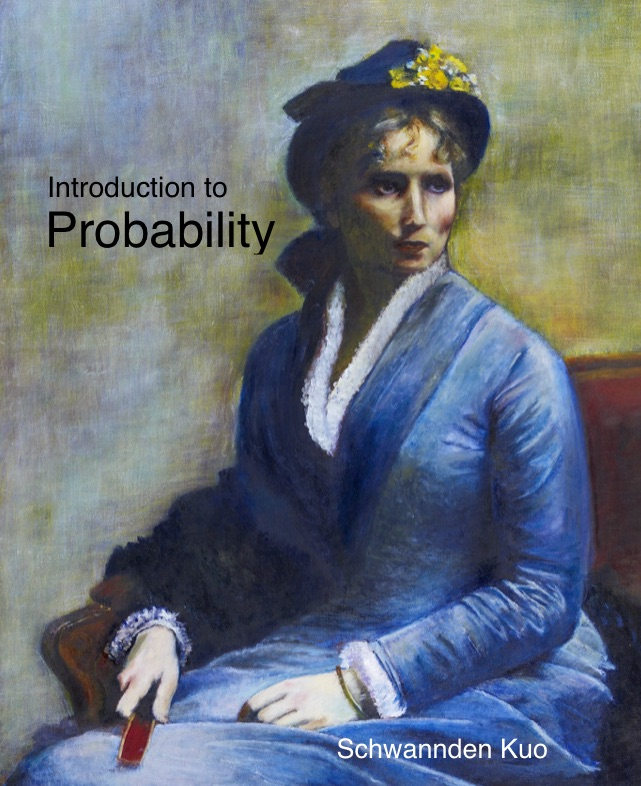
\includegraphics[width=90mm]{charlotteDubourg.jpg}
\\
$$To\ my\ parent,\ Tiger\ and\ Sophie$$
$$Who\ gave\ me\ a\ world\ to\ dream\ and\ always\ encourage\ me\ to\ keep\ dreaming$$
\label{overflow}
\end{figure}

\newpage
\tableofcontents

\newpage
\section{The Notion of Relative Frequency}
The notion of relative frequency can be treated as our starting point of understanding probability. If an experiment has some possible outcomes, but we don't know which outcome will happen (often this property is called "undetermined"). Now how do we define the probability that a particular outcome occur?

One approach is called relative frequency. If we repeat the experiment independently for N times, and obtain our first relative frequency $f_1$ $$f_1 = \frac{\text{number of times a particular event happen}}{N}$$It is hoped that, if we calculate this repeatedly, with $f_n$ be the nth relative frequency,$$\lim_{n\to\infty}\frac{\sum_{i=1}^n f_i}{n} \text{ will converge to a number p}$$We call this $p$ the probability that this particular event happen.

This approach is very intuitive, but the difficulty with this approach is its ambiguity in many aspects, for example:\\
(1) How large should N be?\\
(2) How do we know if the limit exists?\\
(3) How do we know if the limit converges to a single point of a set of point?\\
(4) How fast will relative frequency converge? If it converges too slow, is it still probability?\\

Relative frequency is a good idea, but it is hard to make precise when it comes to proving things mathematically. This is why we need the axiomatic approach \---- we no longer care about the meaning of probability, but the consequence of probability. We no longer ask what is probability, we ask if something has a probability, what properties will this probability have?

This way of studying probability is called an \textbf{axiomatic} approach. It has become a very popular approach for mathematicians to solve problems. You define the consequences of something (called \textbf{axioms}), and if you think these consequences make sense, you derive everything from these simple and basic facts. Physicists use this approach too, but in their world they call it \textbf{laws}, like the three laws of Newton. You can not explain it, you simply accept it. And if one day, a brilliant person find these laws (axioms) unacceptable, and came up with a whole new set of laws (axioms) that explain the world better, then bravo! We got ourselves another Einstein!

An important thing to realize at first is, even though we take the axiomatic approach in this book (rather than a philosophical approach), in the very end, these axioms can prove a theorem called \textbf{the law of large number}. The law of large number basically says that relative frequency will indeed converge to probability. So these axioms \textbf{make sense}!

\newpage
\section{Axiomatic Probability}
\subsection{Sigma Algebra}
Before delving into the axioms of probability, we need to introduce sigma algebra and why we need it.\\

Let $S$ be a sample space, and an event is a subset of $S$. We know probability is a function that maps subset (event) of $S$ to [0,1]. But just what subsets are defined? i.e, what subsets are in the domain of probability function.\\

\textbf{Definition} Let $S$ be a set, and $\Sigma$ is a collection of subsets of $S$.  $\Sigma$ is a sigma algebra  iff\\
(1) There exits some $A \subseteq S$ such that $A\in\Sigma$\\
(2) If $A \in \Sigma$, then $A^c \subset \Sigma$\\
(3) If $A_1, A_2, ... \in \Sigma$, then $\cup_{n=1}^\infty \in \Sigma$\\

Now we say this $\Sigma$ is the domain of probability function.\\

\textbf{Remarks}\\
(a) $2^S$ is obviously a sigma algebra\\
(b) All sigma algebra of $S$ is a subset of $2^S$\\
(c) For property 1 of sigma algebra, we can change it to: $\emptyset \in \Sigma$\\
(d) If $A_1, A_2, ... \in \Sigma$, then $\cap_{n=1}^\infty \in \Sigma$. This can be proved inductively\\

The purpose of $\Sigma$ is that it guarantees the existence of some normal operations of probability. For example, if $\mathbb{P}$ is a probability function, $\mathbb{P}(A)$ and $\mathbb{P}(B)$ exists, one would hope we can find $\mathbb{P}(A \cup B)$ by 
$$\mathbb{P}(A \cup B) = \mathbb{P}(A) +  \mathbb{P}(B) - \mathbb{P}(A \cap B) \ \ \ \ \ \ \ \ \ \ \ \ (1)$$
. The proof that you can find $\mathbb{P}(A \cup B)$ by (1) is easy once you assume the existence of $\mathbb{P}(A \cap B)$, but the existence of $\mathbb{P}(A \cap B)$ is often not guaranteed (i.e, $(A \cap B)$ might not be in the domain of $\mathbb{P}$ ). For example, given a dice, I tell you the probability of throwing out 1 or 3 or 4 is 0.1, and  the probability of throwing out 2 or 3 or 4 is 0.2, can you tell me the probability of throwing out 3 or 4? Of course not (I said of course, but you can prove it more rigorously by yourself)! The properties of sigma algebra guaranteed the existence of such probability, so we can freely use those classical operations about probability.

\subsection{Probability Space}
Probability space is a three tuple
$\{ S, \Sigma,  \mathbb{P}\}$,
where $S$ is sample space, $\Sigma\subseteq 2^S$ is sigma algebra, and $\mathbb{P}: \Sigma \to [0, 1]$ is the probability function such that,\\
(1) $\mathbb{P}(\emptyset) = 0$\\
(2) Given $A_1, A_2, ... \in \Sigma$, if $A_1, A_2, ...$ are mutually exclusive ( $\forall_{i\neq j} A_i \cap A_j = \emptyset$ ), $$\mathbb{P}( \cup_{n=0}^\infty A_n ) = \sum_{n=0}^\infty \mathbb{P}(A_n)$$

\textbf{Definition} We say two events A and B are independent if $\mathbb{P}(A\cap B) = \mathbb{P}(A)\mathbb{P}(B)$

This notion of independence is really the one thing that makes probability a different field of study from analysis. Note in general, $\mathbb{P}(A\cap B) = \mathbb{P}(A)\mathbb{P}(B)$ is not something as a result of a proof, it is usually assumed as premise of a problem, because independence gives probability many useful and convenient properties. 

\subsection{Conditional Probability}
First thing first, \textbf{conditional probability is probability!} As you will next see.

\textbf{Definition} Given probability space $\{ S, \Sigma,  \mathbb{P}\}$, let $A, B$ be two event in $\Sigma$. When we say the conditional probability of A given B, denoted by $\mathbb{P}(A|B) $, we mean the following value $$\mathbb{P}(A\cap B)/\mathbb{P}(B)$$
So the conditional probability given B means the following function:
$$\mathbb{P}(x|B): \Sigma \to [0, 1] \text{ such that } \mathbb{P}(x|B) = \mathbb{P}(x\cap B)/\mathbb{P}(B)$$

Given this definition of conditional probability, we see:\\
(1) $\mathbb{P}(\emptyset|B) = \mathbb{P}(\emptyset\cap B)/\mathbb{P}(B) = \mathbb{P}(\emptyset)/\mathbb{P}(B) = 0$\\
(2) Given $A_1, A_2, ... \in \Sigma$, if $A_1, A_2, ...$ are mutually exclusive, $$\mathbb{P}( \cup_{n=0}^\infty A_n |B ) = \mathbb{P}( (\cup_{n=0}^\infty A_n) \cap B ) /  \mathbb{P}(B)= \mathbb{P}( \cup_{n=0}^\infty (A_n \cap B) ) /  \mathbb{P}(B)$$
$$= \cup_{n=0}^\infty \mathbb{P} ( A_n \cap B ) / \mathbb{P}(B) = \sum_{n=0}^\infty \mathbb{P}(A_n | B)$$\\

So again, \textbf{conditional probability is probability!}\\

With the notion of conditional probability, we can define the notion of independence for events.
\textbf{Definition} We say A and B are independent if $\mathbb{P}(A \cap B) = \mathbb{P}(A) \mathbb{P}(B)$

\textbf{Remark}\\
(a) If $A$ and $B$ are independent event, $\mathbb{P}(A|B) = \mathbb{P}(A)$, which is very intuitive, because the probability of A has nothing to do with B.\\
(b) Even if $A \cap B = \emptyset$, $A, B$ might not be independent.\\
(c) When $\mathbb{P}(B) = 0$, how we define $\mathbb{P}(x|B)$ is up the the application. It's like it is meaningless to define what is $0^0$ unless we are under some application.\\

\newpage
\section{Random Variable}
Sometimes we are not so interested in the sample space, we are more interested in the numerical property of the sample space. For example, if you record the different kinds and number of eagles that fly over Taiwan each day, the sample space consists of some vectors denoting the eagles observed each day.

For example, on June 14th, we add something to the sample space, namely, $$( Crested Goshawk, Spilornis Cheela, Spilornis Cheela, Crested Goshawk )$$
because we observed a Crested Goshawk, followed by two Spilornis cheela, then Crested Goshawk again.

But we might not be interested in the exact form of the record. We might be interested in only how many Crested Goshawk are observed on each day.\\

So we need a way to bring us from sample space to real number, and that thing is called random variable.\\

\textbf{Definition} 
$\mathbb{X}$ is a random variable (r.v) if
$\mathbb{X}: S \to \mathbb{R}$
such that
$$\forall_{t\in\mathbb{R}}\{\mathbb{X}\leq t\}\in \Sigma\ \ \ \ \ \ \ \ \ \ \ (2)$$
, where
$$\{\mathbb{X} \leq t\} \text{ means the set } \{x \in \mathbb{S} | \mathbb{X}(x) \leq t\}$$

So a random variable is a function from sample space to real number. But not all functions from sample space to real number is random variable. We need to be able to ask certain questions about this random variable. 

condition (2) means: if $\mathbb{X}$ is a random variable, I can ask: what is the probability that something happen, and it's value is smaller than $t$. So (2) restricts on the kind of question we can ask about random variable.

Also (2) restrict on the kind of questions we can ask, as the following remark states, we actually can ask just about any question that's realistic.\\

\textbf{Remark}\\
Let $\mathbb{X}$ be a random variable\\
(a) For $A \subset \mathbb{R}$, we denote the set $\{ \mathbb{X} = A \}$ as $\{ x \in S | \mathbb{X}(x) \in A \}$. And if $\{ \mathbb{X} = A \}\in\Sigma$, we say $A$ is "measurable."\\
(b)It can be proved that, 
$$\forall_{t\in \mathbb{R}} \ \ \ \ \ \ \{\mathbb{X} < t \},\ \{\mathbb{X} \geq t \},\ \{\mathbb{X} > t \} \text{ are all measurable}$$\\
(c) With (b), condition (2), we can prove all elementary intervals, namely $(a, b), (a, b], [a, b), [a, b]$, and any countable union or intersection of them, are also measurable.\\

\textbf{Definition} We say two random variables $\mathbb{X}$ and $\mathbb{Y}$ are independent if, $$\forall_{A\text{ measurable } }\mathbb{P}( \{\mathbb{X} = A\} \cap \{\mathbb{Y} = A\} ) = \mathbb{P}(\mathbb{X} = A)\mathbb{P}(\mathbb{Y} = A)$$

\textbf{Definition} We say two random variables $\mathbb{X}$ and $\mathbb{Y}$ are identical if $$\forall_{x\in S}\ \mathbb{X}(x) = \mathbb{Y}(x)$$

\textbf{Definition} We say two random variables $\mathbb{X}$ and $\mathbb{Y}$ are independent, identical distribution if they are independent and identical, denoted i.i.d. This is an acronym that will appear throughout the whole text.

\subsection{Cumulative distribution Function}

\textbf{Definition} Given $\mathbb{X}$, we define the cumulative distribution function (c.d.f) of $\mathbb{X}$ to be $$F(x) = \mathbb{P}\{\mathbb{X} \leq x\}$$

We denote $\mathbb{X}$ has c.d.f $F$ as $\mathbb{X} \sim F(x)$ for brevity. And note that $F$ is defined on $\mathbb{R}$.

Cumulative Distribution Function has some useful properties:\\
(a). c.d.f is right continuous.

\textbf{Proof}

From calculus, we know
\begin{center}
 $\lim_{n\to\infty}f(x_n)=f(x) $for any sequence $\{x_n\}$ such that $x_n \to x$\\ 
\textbf{if and only if}\\
 $\lim_{t\to x}f(t)=f(x)$
\end{center}
 
And for any $\{x_n\}$ in $[x, \infty )$ such that $x_n\to x$, and let $A_n$ be $(-\infty, x_n]$
$$F(\mathbb{X}\leq x) = \mathbb{P}( \mathbb{X} = \cap_{n=1}^\infty A_n )
 \text{\ \ \ (because   } (-\infty, x] = \cap_{n=1}^\infty A_n )$$
$$= \mathbb{P}(\cap_{n=1}^\infty\{\mathbb{X} = A_n \}) = \cap_{n=1}^\infty\mathbb{P}(\mathbb{X} = A_n ) = \lim_{n\to\infty}\mathbb{P}(\mathbb{X} = A_n ) = \lim_{n\to\infty}\mathbb{P}(\mathbb{X} \leq x_n )$$

The choice of $\{x_n\}$ was arbitrary, so $$\forall_x \lim_{t\to x^+}F(t) = F(x)$$\\
(b). c.d.f is non-decreasing.\\
(c). $\lim_{t\to \infty}F(t) = 1, \lim_{t\to -\infty}F(t) = 0$\\
(d). If $a<b$, $\mathbb{P}( \mathbb{X}\leq b ) = \mathbb{P}( \mathbb{X} \leq a ) + \mathbb{P}( a < \mathbb{X} \leq b )$ (because $\{\mathbb{X}\leq a\}$ and $\{a<\mathbb{X}\leq b\}$ are disjoint set), so $$\mathbb{P}( a < \mathbb{X} \leq b ) = F(b) - F(a)$$

C.d.f and its properties are often useful, because it is independent of the different types of random variable. These properties are true as long as it is a c.d.f of a random variable.

\subsection{Conditional Random Variable}
Just like in probability, We want to see what happens if probability of an event is conditioned on some other event, we want to know about conditioning random variable.
First thing first, \textbf{conditional random variable is random variable!}\\

\textbf{Definition} Let $\mathbb{X}, \mathbb{Y}$ be two random variable. When we say the conditional random variable of $\mathbb{X}$ given $\mathbb{Y} = y$, denoted by $\mathbb{X}|{\mathbb{Y}=y} $, we mean the random variable that has the following c.d.f:
$$F_{X|Y}(x|Y=y) = \frac{\mathbb{P}( \{\mathbb{X} \leq x\} \cap \{\mathbb{Y} = y\} )}{\mathbb{P}(\mathbb{Y} = A)} $$

And we call this $F_{X|Y}(x|Y=y)$ the conditional c.d.f of $\mathbb{X}$ given $\mathbb{Y} = y$

In chapter 4, we will see if two random variables has joint c.d.f, there is a formula for calculating $F_{X|Y}$.

\subsection{Types Of Random Variable}
Some times we want to know the probability when a random variable have a certain value. For example, if you toss a coin, and we let $\mathbb{X}$ be a random variable such that it is 1 if the coin is head, and 0 otherwise. It is fairly understandable that we would want to know $\mathbb{P}(\mathbb{X} = 1)$ or $\mathbb{P}(\mathbb{X} = 0)$. But sometimes it is not so intuitive to tell people the exact meaning of $\mathbb{P}(\mathbb{X} = a)$, where $a$ is some constant. For example, if you are predicting tomorrow's average temperature, what is the probability that it will be exactly 20 degree Celsius? Supposedly it is very unlikely because it might be 20.0000001, 19.9999999 or 
maybe some other not-so-close answer. But you won't say it is impossible either, because there is always a chance that it turns out to be exactly 20 degree. The problem here, is that this random variable (tomorrow's average temperature) takes on infinitely many values. Although some values are more likely than the others, every single point is very unlikely.\\

This is when we need to distinguish very clearly the two kind of different random variables, discrete and continuous. And we use different approaches to define what does it mean by $\mathbb{P}(\mathbb{X} = a)$.

\subsubsection{Discrete Random Variable}
\textbf{Definition}
We say a random variable $\mathbb{X}$ is discrete if the range of $\mathbb{X}$ is at most countable, and we define probability mass function (p.m.f) of $\mathbb{X}$ to be
$p(x) = \mathbb{P}\{\mathbb{X}=x\}$, denoted $\mathbb{X} \sim p(x)$

This is very straight forward, because $\mathbb{P}\{\mathbb{X}=x\}$ is, well, $\mathbb{P}\{\mathbb{X}=x\}$. There really is no need for other fancy method.\\

\textbf{Remark}
If $\mathbb{X}$ is discrete r.v with p.d.f $p(x)$ and p.m.f $F(x)$\\
(a) The sample space $S$ need not be at most countable, only the range of $\mathbb{X}$ need to be at most countable.\\
(b) $p(x) > 0$ for at most countable point, because the range of $\mathbb{X}$ is at most countable.\\
(c) $$F(x) = \sum_{t\leq x, p(t)>0}p(t)$$
Here, we cannot simply sum $p(t)$ over all $t\leq x$, because the number of $t\leq x$ might be uncountable.


\subsubsection{Continuous Random Variable}
\textbf{Definition} We say a real function $F$ is absolutely continuous if there exists real function $f$ such that
$$\forall_a \forall_x \ \ F(x) = f(a) + \int_a^x f(t) \mathrm{d}t$$

\textbf{Definition}
We say a random variable $\mathbb{X} \sim F$ is continuous if its c.d.f $F$ is absolutely continuous\\

\textbf{Definition}
The function $f$ such that $\forall_a \forall_x \ \ F(x) = f(a) + \int_a^x f(t) \mathrm{d}t$ is called the probability density function (p.d.f) of $\mathbb{X}$.\\

Now let's take a look at the probability mass function of $\mathbb{\mathbb{X}}$.

For any number $a\in\mathbb{R}$, let $A_n$ be the half open interval $(a-\frac{1}{n}, a]$
$$\mathbb{P}(\mathbb{X}=a) = \mathbb{P}( \mathbb{X} = \cap_{n=1}^\infty A_n )
 \text{\ \ \ (because   } a = \cap_{n=1}^\infty A_n )$$
$$= \mathbb{P}(\cap_{n=1}^\infty\{\mathbb{X} = A_n \}) = \cap_{n=1}^\infty\mathbb{P}(\mathbb{X} = A_n )$$ where the last equality comes from the continuity of probability function on monotonic sequence of sets. Now
$$\cap_{n=1}^\infty\mathbb{P}(\mathbb{X} = A_n ) = \cap_{n=1}^\infty F(a) - F(a-\frac{1}{n}) = \lim_{n\to\infty} F(a) - F(a-\frac{1}{n})$$

If $\mathbb{X}$ is continuous r.v,  then
$$\mathbb{P}(\mathbb{X}=a) = \lim_{n\to\infty} F(a) - F(a-\frac{1}{n}) = 0$$
because $F$ is continuous.

Therefore, p.m.f of a continuous r.v is meaningless, because it's p.m.f is 0 every where. So p.d.f is what we need to capture the spirit of $\mathbb{P}\{\mathbb{X}=x\}$, even though $\mathbb{P}\{\mathbb{X}=x\}$ is $0$.
\textbf{Remark}\\
(1)When something has a probability 0, it doesn't mean it won't happen! As we just see, any p.m.f of a contunuous random variable is 0.\\
(2)Given a c.d.f $F$, its corresponding p.d.f $f$, is not unique. However, it rarely matters because the results we need generally come from imtergrating $f$, and even if there are differen $f$'s, the result after intergrating is always the same. Why? To answer this you will have to take some courses in measure theory.

\subsection{Expectation}
Expectation is a way to characterize a random variable.\\

\textbf{Definition} Let $g$ be a real function, the expectation of a random variable $\mathbb{X} \sim f$, denoted $\mathbb{E}[g(\mathbb{X})]$, is defined as
$$
\mathbb{E}[g(\mathbb{X})] =
  \begin{cases}
   \sum_{x|f(x)>0} g(x)f(x) & \text{ for discrete random variable}\\
   \int_{-\infty}^{\infty} g(x)f(x) \mathrm{d}x & \text{ for continuous random variable}
  \end{cases}
$$
Note here $f$ is treated as p.m.f in discrete case and p.d.f in continuous case.\\

In the special case $g(x) = x$, $\mathbb{E}[g(\mathbb{X})] = \mathbb{E}[\mathbb{X}]$ is called the \textbf{mean} of $\mathbb{X}$, usually denoted by $\mu$. And in the special case that $g(x) = (x-\mu)^2$, $\mathbb{E}[g(\mathbb{X})] = \mathbb{E}[(\mathbb{X}-\mu)^2]$ is called the \textbf{variance} of $\mathbb{X}$, usually denoted by $\sigma^2$\\

Some properties of mean and variance:\\
(a) For any constant $a$, $\mathbb{E}[a] = a$. This follows from the fact that ${\sum_{x|f(x)>0}f(x) = 1}$ in discrete case, and ${\int_{-\infty}^{\infty}f(x)\mathrm{d}x = 1}$ in continuous case.\\
(b) For any constants $a, b$, $\mathbb{E}[a\mathbb{X}+b] = a\mathbb{E}[\mathbb{X}]+b$, provided that $\mathbb{E}[\mathbb{X}]$ exists. The proof follows from the fact that we can take scalar out of a convergent integral and series.\\
(c) Let $\sigma^2$ be the variance of $\mathbb{X}$, the variance of $a\mathbb{X}$ is $a^2\sigma^2$, the proof is trivial.\\
(d) $\sigma^2 = \mathbb{E}[(\mathbb{X}-\mu)^2] = \mathbb{E}[\mathbb{X}^2]-2\mu\mathbb{E}[\mathbb{X}]+\mathbb{E}[\mu^2] = \mathbb{E}[\mathbb{X}^2] - \mu^2$


\subsection{Moment Generating Function}
The moment generating function (m.g.f) of a random variable $\mathbb{X}$, denoted $M_X(t)$, is defined as
$$M_X(t) = \mathbb{E}[e^{\mathbb{X}t}]\text{ provided the expectation exists}$$

Moment generating function is very useful in finding out some properties of a random variable. As the following two theorems shows how can we find the means of a random variable by its m.g.f.\\

\textbf{Theorem} If $\mathbb{X} \sim p$ is a discrete random variable with finite range, Then $M_X'(0) = \mu$.\\

\textbf{Theorem} If $\mathbb{X} \sim p$ is a discrete random variable with infinite range, $x_1, x_2, ...$ is the sequence of all points in the range of $\mathbb{X}$, and let $g_n(t) = e^{x_n t}p(x_n)$. Now if there exists $\epsilon$ such that\\
(1) $\sum_{n=1}^\infty g_n(t)$ converges for some $t$ in a $[0-\epsilon, 0+\epsilon]$\\
(2) $\sum_{n=1}^\infty g_n'(t)$ converge absolutely in $[0-\epsilon, 0+\epsilon]$\\

Then $M_X'(0) = \mu$.\\

\textbf{Theorem} If $\mathbb{X} \sim f$ is a continuous random variable, let $g(x, t) = e^{x t}f(x)$.\\
(1) There exists a closed interval $A$ such that $0 \in A$ and for all $t \in A$, $M_X(t)$ exist\\
(2) For every $\epsilon > 0$ there exists $\delta$ such that $| \mathrm{D}_t g(x, t) - \mathrm{D}_t g(x, s) | < \epsilon$ for all $x$ and for all $|s-t|\leq\delta$\\

Then $M_X'(0) = \mu$.\\

\textbf{Proof to both} If the conditions are satisfied,
$$M_X'(0) = \frac{\mathrm{d}}{\mathrm{d} t}\mathbb{E}[e^{\mathbb{X}t}] |_{t=0} = \mathbb{E}[ \frac{\mathrm{d}}{\mathrm{d} t} e^{\mathbb{X}t}] |_{t=0} = \mathbb{E}[\mathbb{X}] = \mu$$
We can take the differentiation into expectation because the theorems in analysis tells us we can interchange differentiation with infinite summation or differentiation with integration if conditions 1, 2 are satisfied (See appendix for under what conditions are we allowed to do so).\\

\textbf{Definition} The nth moment of a random variable $\mathbb{X}$ is defined as $\mathbb{E}[\mathbb{X}^n]$\\

Reader should be able to varify that $M_X^{(n)}(0) = \mathbb{E}[\mathbb{X}^n]$ (under appropriate conditions), so that $\sigma^2 = M_X''(0) - (M_X'(0))^2$ provides a nother way tp caluculate variance via moment generating function.\\

\textbf{Theorem} Uniquess Property of Moment gGenerating Function.
$$M_X(t) = M_Y(t) \text{ if and only if } \mathbb{X}=\mathbb{Y}$$

This is the first theorem you encounter in this textbook that I shall not give it a proof. Because the proof concept is beyond basic analysis.


\newpage
\section{Some Example Distributions}
\subsection{Example Discrete Random Variable}
\subsubsection{Bernoulli Random Variable}
\textbf{Definition} We say a discrete random variable $\mathbb{X}$ is a Bernoulli random variable with parameter $p$, or has a Bernoulli distribution with parameter $p$, denoted by $\mathbb{X} \sim Bernoulli(p)$ if
$$
 \mathbb{X} \sim p(n) =
  \begin{cases}
   p & \text{if } n = 1 \\
   1-p       & \text{if } n = 0
  \end{cases}
$$\\

For $\mathbb{X} \sim Bernoulli(p)$, $\mu = p$, and $\sigma^2 = p(1-p)$\\

\textbf{Property} If $\mathbb{X} \sim Bernoulli(p)$, then $\mu = p, \sigma^2 = p(1-p)$\\

\textbf{Proof 1}
By definition, trivial\\

\textbf{Proof 2}
Since $\mathbb{X}$ has finite range, and there is no problem in interchanging limit and finite summation, we can find $\mu$ and $\sigma$ via m.g.f.
$$M_X(t) = \mathbb{E}[e^{\mathbb{X}t}] = pe^{1*t} + (1-p)e^{0*t} = pe^t$$
So $\mu = M_X'(0) = p$, $\sigma^2 = M_X''(0) - (M_X'(0))^2 = p-p^2 = p(1-p)$

\subsubsection{Binomial Random Variable}
\textbf{Definition} We say a discrete random variable $\mathbb{X}$ is a binomial random variable with parameter $n, p$, or has a binomial distribution with parameter $n, p$, denoted by $\mathbb{X} \sim binomial(n, p)$ if
$$
 \mathbb{X} \sim p(k) =
  \begin{cases}
   {n \choose k}p^k(1-p)^{n-k} & \text{if } k \in \{0, 1, 2, ..., n\} \\
   1-p       & \text{otherwise}
  \end{cases}
$$\\

This random variable happens if we have n i.i.d Bernoulli(p).\\

For $\mathbb{X} \sim binomial(n, p)$, $\mu = np$, and $\sigma^2 = np(1-p)$\\

\textbf{Property} If $\mathbb{X} \sim binomial(n, p$, then $\mu = np, \sigma^2 = np(1-p)$\\

\textbf{Proof 1} By definition

Firstly note that
$$\mathbb{E}[X^m] = \sum_{k=0}^n k^m {n \choose k}p^k(1-p)^{n-k} = np \sum_{k=0}^n k^{m-1} \frac{(n-1)!}{(k-1)!(n-k)!}p^{k-1}(1-p)^{n-k}$$
$$= np \sum_{k=1}^n k^{m-1} \frac{(n-1)!}{(k-1)!(n-k)!}p^{k-1}(1-p)^{n-k} = np \sum_{k=0}^{n-1} (k+1)^{m-1} \frac{(n-1)!}{k!(n-k-1)!}p^{k-1}(1-p)^{n-k}$$
$$= np \sum_{k=0}^{n-1} (k+1)^{m-1} {n-1 \choose k}p^k(1-p)^{n-k} = np(\mathbb{E}[\mathbb{Y}+1)^{m-1}]$$
where $\mathbb{Y} \sim binomial(n-1, p)$\\

So $\mu = np \mathbb{E}[1] = np$, and $\sigma^2 = \mathbb{E}[\mathbb{X}^2] - \mu^2 = np\mathbb{E}[\mathbb{Y}+1)] - n^2p^2 = np((n-1)p + 1) - n^2p^2 = np(1-p)$\\

\textbf{Proof 2}
Here we can find $\mu$ and $\sigma$ via m.g.f because $\mathbb{X}$ has finite range.

The moment generating function
$$M_x(t) = \mathbb{E}[e^{\mathbb{X}t}] = \sum_{k=0}^n e^{kt} {n \choose k}p^k(1-p)^{n-k} = (1-p+pe^t)^n$$
So the mean
$$ \mu = \mathbb{E}[\mathbb{X}] = M_x'(0) = n (1-p+pe^t)^{n-1} pe^t |_{t=0}= np$$
and variance
$$\sigma^2 = \mathbb{E}[\mathbb{X}^2] - \mathbb{E}[\mathbb{X}]^2 = M_X''(0) - \mu^2 = np + n(n-1)p^2 - n^2p^2 = np(1-p) $$ 

\subsubsection{Poisson Random Variable}
\textbf{Definition} We say a discrete r.v $\mathbb{X}$ is a Poisson r.v with parameters $\lambda$, denoted $\mathbb{X} \sim poisson(\lambda)$, if
$$
 \mathbb{X} \sim p(n) =
  \begin{cases}
   \frac{\lambda^n}{n!}e^{-\lambda} & \text{if } n \in 0, 1, 2, 3... \\
   0       & \text{otherwise}
  \end{cases}
$$\\

\textbf{Property} If $\mathbb{X} \sim posson(\lambda)$, then $\mu = \sigma^2 = \lambda$\\

\textbf{Proof 1} By definition
$$\mathbb{E}[\mathbb{X}] = \sum_{n=0}^\infty n\frac{\lambda^n}{n!}e^{-\lambda} = \lambda \sum_{n=1}^\infty \frac{\lambda^{n-1}}{(n-1)!}e^{-\lambda} = \lambda$$
$$\mathbb{E}[\mathbb{X}^2] = \sum_{n=0}^\infty n^2\frac{\lambda^n}{n!}e^{-\lambda} = \lambda \sum_{n=1}^\infty n  \frac{\lambda^{n-1}}{(n-1)!}e^{-\lambda} =  \lambda \sum_{n=0}^\infty (n+1)  \frac{\lambda^{n}}{n!}e^{-\lambda} = \lambda (\mathbb{E}[\mathbb{X}] + 1)$$
so $var(\mathbb{X}) = \mathbb{E}[\mathbb{X}^2] - (\mathbb{E}[\mathbb{X}])^2 = \lambda$\\

\textbf{Proof 2} By moment generating function\\

First lets check if it is eligible to apply moment generating function.\\
(a) $\frac{\mathrm{d}}{\mathrm{d}t} f(n)e^{nt} = \frac{\lambda^n}{(n-1)!}e^{-\lambda}e^{nt}$, $\sum_{n=1}^\infty \frac{\lambda^n}{(n-1)!}e^{-\lambda}e^{nt} = \lambda e^{t-\lambda} \sum_{n=0}^\infty \frac{(\lambda e^t)^n}{n!}$. 

$= \lambda e^{\lambda e^t + t - \lambda}$. This convergence is definitely uniform for some closed interval containing $0$ (In fact, this convergence is uniform for all closed interval, see appendix for uniform convergence property on power series).\\
(b) $\sum f(n)e^{nt} = \sum_{n=0}^\infty e^{nt}  \frac{\lambda^n}{n!}e^{-\lambda} = e^{-\lambda} \sum_{n=0}^\infty \frac{ (\lambda e^t)^n}{n!} = e^{\lambda (e^t - 1)}$ converges on all points\\

Since (a), (b) hold, $\mu = M_X'(0)$. $M_X(t) = e^{\lambda (e^t - 1)}$ as (b) already showed, so the mean
$ \mu = M_x'(0) = \lambda e^t e^{\lambda (e^t - 1)} |_{t=0} = \lambda $
and variance
$$\sigma^2 = \mathbb{E}[\mathbb{X}^2] - \mathbb{E}[\mathbb{X}]^2 = M_X''(0) - \mu^2 = \lambda + \lambda^2 - \lambda^2 = \lambda$$

\subsection{Example Continuous Random Variable}
\subsubsection{Uniform Random Variable}
\textbf{Definition} We say a continuous random variable $\mathbb{X}$ is a uniformly distributed in [a, b], denoted $\mathbb{X} \sim uniform(a, b)$ if
$$
 \mathbb{X} \sim f(x) =
  \begin{cases}
   \frac{1}{b-a} & \text{if } x \in [a, b] \\
   0       & \text{otherwise}
  \end{cases}
$$\\

\textbf{Property} If $\mathbb{X} \sim uniform(a, b)$, then $\mu = \frac{a+b}{2}, \sigma^2 = \frac{(b-a)^2}{12}$\\

\textbf{Proof 1} By definition
$\mu = \int_a^b \frac{x}{b-a} \mathrm{d}x = \frac{a+b}{2}$,\\ $\sigma^2 = \int_a^b \frac{x^2}{b-a} \mathrm{d}x - (\frac{a+b}{2})^2 = \frac{b^2+ab+a^2}{3} - \frac{a^2+2ab+b^2}{4} = \frac{(b-a)^2}{12}$\\

\textbf{Proof 2} By moment generating function\\

Since $D_t f(x)e^{xt} = D_t \frac{e^{xt}}{b-a} = \frac{xe^{xt}}{b-a}$ is continuous on $\mathbb{R}^2$, and\\
$M_X(t) = \int_a^b \frac{e^{xt}}{b-a} \mathrm{d}x = 
\begin{cases}
\frac{e^{bt}-e^{at}}{t(b-a)} & \text{ if } t \neq 0\\
1 & \text{ if } t = 0
\end{cases}$ exists for all $t$, all conditions that garantee the valiidty of m.f.g method can be met.\\
so
$$\mu = M_X'(0) = \lim_{t\to 0} \frac{1}{t}( \frac{e^{bt}-e^{at}}{t(b-a)} - 1 ) = \lim_{t\to 0} \frac{e^{bt}-e^{at}-t(b-a)}{t^2(b-a)}$$
$$\text{ (apply L'hospital twice) }= \lim_{t\to 0} \frac{b^2e^{bt}-a^2e^{at}}{2(b-a)} = \frac{a+b}{2} $$
And
$$M_X''(0) = \lim_{t\to 0} \frac{1}{t}( \frac{t(b-a)(be^{bt}-ae^{at})-(e^{bt}-e^{at})(b-a)}{t^2(b-a)^2} - \frac{a+b}{2} )$$
$$= \lim_{t\to 0} \frac{2t(b-a)(be^{bt}-ae^{at})-2(e^{bt}-e^{at})(b-a) - (a+b)t(b-a)^2)}{2t^3(b-a)^2}$$
$$\text{ (apply L'hospital 3 times ) }= \frac{4(b-a)(b^3-a^3)}{12(b-a)^2} = \frac{a^2 + ab + b^2}{3}$$

So $\sigma^2 = \frac{a^2 + ab + b^2}{3} - (\frac{a+b}{2})^2 = \frac{(b-a)^2}{12}$

\subsubsection{Normal Random Variable}
\textbf{Definition} We say a continuous random variable $\mathbb{X}$ is has a normal distribution with parameter $\mu, \sigma^2$, denoted $\mathbb{X} \sim normal(\mu, \sigma^2)$ if
$$
 \mathbb{X} \sim f(x) = \frac{1}{\sqrt{2\pi}\sigma}e^{-\frac{(x-\mu)^2}{2\sigma^2}}
 \text{ for all } x\in\mathbb{R}
$$

\textbf{Property} If $\mathbb{X} \sim normal(\mu, \sigma^2)$, then $\mu$ is the mean and $\sigma^2$ is the variance\\

\textbf{Proof 1} By definition

First note that if $\mathbb{X} \sim normal(\mu, \sigma^2)$, then $\mathbb{X} = \sigma\mathbb{Z}+\mu$, where $\mathbb{Z}$ is standard normal distribution, with $\mu = 0, \sigma = 1$. So we only need to prove that the mean and variance of $\mathbb{Z}$ is $0$ and $1$, (to see why $\mathbb{X} = \sigma\mathbb{Z}+\mu$, look at their c.d.f).

$$\mathbb{E}[\mathbb{Z}] = \int_{-\infty}^\infty \frac{x}{\sqrt{2\pi}} e^{-\frac{x^2}{2}}\mathrm{d}x = 0 \text{ because } \frac{x}{\sqrt{2\pi}} e^{-\frac{x^2}{2}} \text{ is odd and the integration exists}$$
$$\text{variance of } \mathbb{Z} = \int_{-\infty}^\infty \frac{x^2}{\sqrt{2\pi}} e^{-\frac{x^2}{2}}\mathrm{d}x = \int_{-\infty}^\infty x * \frac{x}{\sqrt{2\pi}} e^{-\frac{x^2}{2}}\mathrm{d}x$$
$$\text{(integration by part) } = 0 + \frac{1}{\sqrt{2\pi}} \int_{-\infty}^\infty e^{-\frac{x^2}{2}}\mathrm{d}x = 1$$
Here we used the identity $\int_{-\infty}^\infty e^{-\frac{x^2}{2}}\mathrm{d}x = \sqrt{2\pi}$\\

\textbf{Proof 2} By moment generating function\\

Since $D_t (f(x)e^{xt}) = xe^{xt}e^{-\frac{(x-\mu)^2}{2\sigma^2}}$ is continuous on $\mathbb{R}^2$, we can use m.g.f method.

The moment generating function
$$M_x(t) = \mathbb{E}[e^{\mathbb{X}t}] = \int_{-\infty}^\infty e^{xt} \frac{1}{\sqrt{2\pi}\sigma}e^{-\frac{(x-\mu)^2}{2\sigma^2}} \mathrm{d}x = \frac{1}{\sqrt{2\pi}\sigma} \int_{-\infty}^\infty e^{-\frac{(x-\mu)^2-2 \sigma^2 t x}{2\sigma^2}} \mathrm{d}x$$

$$= \frac{1}{\sqrt{2\pi}\sigma} e^{\frac{(\mu+\sigma^2 t)^2 - \mu^2}{2\sigma^2}} \int_{-\infty}^\infty e^{-\frac{(x-(\mu+\sigma^2 t))^2}{2\sigma^2}} \mathrm{d}x = e^{\frac{2\mu\sigma^2 t+\sigma^4 t^2 }{2\sigma^2}} = e^{\frac{\sigma^2 t^2}{2}+\mu t}$$
So the mean
$$ \mu = \mathbb{E}[\mathbb{X}] = M_x'(0) = (\sigma^2 t + \mu) e^{\frac{\sigma^2 t^2}{2}+\mu t} |_{t=0} = \mu$$
and variance
$$\sigma^2 = M_X''(0) - \mu^2 = (\sigma^2 t + \mu)^2 e^{\frac{\sigma^2 t^2}{2}+\mu t} + \sigma^2 |_{t=0} - \mu^2 = \sigma^2$$


\subsubsection{Exponential Random Variable}
\textbf{Definition} We say a continuous random variable $\mathbb{X}$ is has a exponential distribution with parameter $\lambda$, denoted $\mathbb{X} \sim exp(\lambda)$ if
$$
\begin{cases}
 \mathbb{X} \sim f(x) = \lambda e^{-\lambda x} & \text{if } x \geq 0\\
 0 & \text{otherwise}
 \end{cases}
$$

\textbf{Property} If $\mathbb{X} \sim exp(\lambda)$, $\mu = \frac{1}{\lambda}, \sigma^2 = \frac{1}{\lambda^2}$\\

\textbf{Proof 1} By definition\\
$$\mathbb{E}[\mathbb{X}] = \int_0^\infty \lambda x e^{-\lambda x} \mathrm{d}x = [-xe^{-\lambda x}]_0^\infty + \int_0^\infty e^{-\lambda x} \mathrm{d}x = \frac{1}{\lambda}$$
And since $\mathbb{E}[\mathbb{X}^2] = \int_0^\infty \lambda x^2 e^{-\lambda x} \mathrm{d}x = [-x^2e^{-\lambda x}]_0^\infty + \int_0^\infty 2xe^{-\lambda x} \mathrm{d}x = \frac{2}{\lambda^2}$
$$\sigma^2 = \mathbb{E}[\mathbb{X}^2] - \mu^2 = \frac{1}{\lambda^2}$$


\textbf{Proof 2} By moment generating function\\
Since $D_t (\lambda e^{-\lambda x} e^{xt}) = \lambda x e^{(t-\lambda) x}$ is continuous on $(-\lambda, \lambda ) \times [0, \infty)$, we can apply m.g.f method.

$M_X(t) = \int_0^\infty \lambda e^{-\lambda x} e^{xt} \mathrm{d}x = \int_0^\infty \lambda e^{(t-\lambda) x} \mathrm{d}x = [\frac{\lambda}{t-\lambda}]_{t = 0}^\infty = \frac{\lambda}{\lambda - t}$ so
$$\mu = M_X'(0) = \frac{\lambda}{(\lambda - t)^2} |_{t=0} = \frac{1}{\lambda}$$
$$\sigma^2 = M_X''(0) - \mu^2 = \frac{2\lambda}{(\lambda - t)^3} |_{t=0} - \frac{1}{\lambda^2} = \frac{1}{\lambda^2}$$


\subsubsection{Beta Random Variable}
\textbf{Definition} of $beta function$: if $x>0$ and $y>0$, the $beta function$ is
$$B(x, y) = \int_0^1 t^{x-1}(1-t)^{y-1}\mathrm{d}t$$ 

We say a continuous r.v $\mathbb{X}$ is a beta r.v with parameters $x, y$, denoted $\mathbb{X} \sim \beta(x, y)$, if
$$
 \mathbb{X} \sim f(x) =
  \begin{cases}
   \frac{1}{B(x, y)} t^{x-1} (1-t)^{y-1} & \text{if } x > 0, y>0 \\
   0       & otherwises
  \end{cases}
$$

The follow question shows how $beta$ distribution might arise:\\

\textbf{Example} If we know the probability of an experiment being successful is p, p exits but unknown. We also know that the value of p is a uniform distribution in [0,1]. So we decide to do the experiment n+m times and we found out that n of which turned out successful. Now what do we know about the distribution of p?\\

\textbf{Solution}
Let $E_1, E_2, ..., E_{m+n}$ be i.i.d Bernoulli(p), where $E_i$ is 1 if the ith experiment turns out successful and 0 otherwise. Given $P \sim uniform(0, 1)$ and $N = \sum_{i=1}^n E_i \sim binomial(m+n, p)$, the conditional c.d.f 
$$F_{P|N}(p|\mathbb{N}=n) = \frac{\mathbb{P}( \{P \leq p\} \cap \{\mathbb{N} = n\} )}{\mathbb{P}(\mathbb{N} = n)} = \frac{\mathbb{P}( \mathbb{N} = n | P \leq p )\  \mathbb{P}( P \leq p )}{\mathbb{P}(\mathbb{N} = n)} $$
$$= \frac{\int_0^p \mathbb{P} (\mathbb{N} = n | P=p) \mathrm{d}p \  \mathbb{P}( P \leq p )}{\int_0^1 \mathbb{P} (\mathbb{N} = n | P=p) \mathrm{d}p }$$
$$\Rightarrow f_{P|N}(p|\mathbb{N}=n) = F'_{P|N}(p|\mathbb{N}=n) =   \frac{\mathbb{P} (\mathbb{N} = n | P=p)\ f_P(p)}{\int_0^1 \mathbb{P} (\mathbb{N} = n | P=p) \mathrm{d}p }$$
$$= \frac{ {n+m \choose n}p^n(1-p)^m }{\int_0^1{ n+m \choose n}p^n(1-p)^m\mathrm{d}p} = \frac{1}{B(n+1, m+1)} p^n (1-p)^m$$
And this is exactly the p.d.f for $beta(n+1, m+1)$.\\

\textbf{Example} $X_1, .., X_n \overset{i.i.d}{\sim} uniform(0, 1), Y_1 = X_{(1)} (min( X_1, ..., X_n )), Y_n = X_{(n)}$, shoe that $Y_1 \sim beta(1, n), Y_n \sim beta(n, 1)$\\

\textbf{Solution}
$F_{Y_n}(y) = \mathbb{P}(X_1 \leq y, ..., X_n \leq y) = y^n $ for $y \in [0, 1]$, so $f_{Y_n}(y) = ny^{n-1} = \frac{1}{B(n, 1)}y^{n-1} \sim beta(n, 1)$ for $y \in [0, 1]$. $F_{Y_1}$ can be shown similarly, with $F_{Y_1}(y) = 1-(1-y)^n$, and $f_{Y_1} = n(1-y)^{n-1}$

\subsubsection{Gamma random variable}
\subsubsection*{Introducing gamma function}
\textbf{Definition} The $gamma function$ is defined as
{\center}$$\Gamma(x) = \int_0^{\infty} t^{x-1}e^{-t} \mathrm{d}t\ \ \ \ \ \ \ \ \ \ (1)$${\center} 
for all $x > 0$ \\

Note that $\Gamma$ converge if and only if $x>0$, as the following analysis shows:\\

If $x>0$,  $$\lim_{t\rightarrow\infty} \frac{t^{x-1}e^{-t}}{e^{-t/2}} = 0$$

this means $$ \exists_m \forall_{t\geq m}  t^{x-1}e^{-t} \leq {e^{-t/2}} $$

And by comparison test, $\int_m^{\infty} t^{x-1}e^{-t} \mathrm{d}t$ exists.

Now if $x > 1$,  $\int_0^m t^{x-1}e^{-t} \mathrm{d}t$ is just a definite integral, so $\Gamma$ converges for $x>1$. If $x=1$, $\Gamma(1) = 1$ by directly evaluating the indefinite integral.

If $x<1$, $t^{x-1}e^{-t} \leq t^{x-1}$, and we know $\int_0^m t^{x-1} \mathrm{d}t$ converges iff $x-1>-1$, i.e, $x>0$. By comparison test, we know $\Gamma$ converges for $x>0$.

If $x=0$, integration by part shows $\Gamma$ diverge, then comparison test can show that for all $x<0$ $\Gamma$ diverge.\\

\textbf{Some properties of $\Gamma$:}\\
(a) for all $0<x<\infty$, $\Gamma(x+1) = x\Gamma(x)$ \\
(b) $\Gamma(n+1) = n!$\\
(c) $\log \Gamma$ is convex on $(0, \infty)$\\
We say a real function $f$ is convex on $A$ if and only if for every $x, y\in A$, and $\lambda \in [0.1]$, $f(\lambda x + (1-\lambda)y) \leq \lambda f(x) + (1-\lambda)f(y)$\\

(a) can be shown with integration by part, and (b) can be shown by first find out $\Gamma(1)=1$, then apply (a). for (c), we need Holder's inequality:
{\center}
If $f$ and $g$ are Riemann integrable real functions on $[a, b]$, for any $p$, $q$ s.t $\frac{1}{p} + \frac{1}{q} = 1$
$$|\int_a^b fg\ \mathrm{d}\alpha| \leq {\int_a^b |f|^{\frac{1}{p}}\mathrm{d}\alpha}^p {\int_a^b |g|^{\frac{1}{q}}\mathrm{d}\alpha}^q\ \ \ \ \ \ \ \ \ \ (2) $$
{\center}

With this inequality, 
$$\Gamma(\frac{x}{p} + \frac{y}{q}) = 
\int_0^\infty t^{\frac{x}{p} + \frac{y}{q} - 1}e^{-t} \mathrm{d}t = 
\int_0^\infty (t^\frac{x-1}{p}e^{-\frac{t}{p}}) (t^\frac{y-1}{q}e^{-\frac{t}{q}}) \mathrm{d}t \leq \Gamma(x) ^ {\frac{1}{p}} \Gamma(y) ^ {\frac{1}{q}}$$

Therefore
$$\log\Gamma( \frac{x}{p} + \frac{y}{q} ) \leq \frac{1}{p}\log\Gamma(x)+ \frac{1}{q}\log\Gamma(y)$$ 

Now it is actually very cool that these 3 properties uniquely determines $\Gamma$, as the following theorem shows.\\

\textbf{theorem 1}\ \ \ \ 
Let $f$ be a real function defined  on $(0, \infty)$, such that:

(a) for all $0<x<\infty$, $f(x+1) = xf(x)$ 

(b) $f(1) = 1$

(c) $\log f$ is convex on $(0, \infty)$

then f is uniquely determined. This says, f is $\Gamma$, since $\Gamma$ satisfies all three properties.\\

\textbf{proof} Let $\varphi$ be $\log f$. first note $\varphi(x+1) = \varphi(x) + \log(x)$. Since $\varphi$ is convex, 
$\forall n \in \mathbb{N}\ \forall x \in (0, 1)$ $$ \varphi(n+1)-\varphi(n) \leq\frac{\varphi(n+1+x)-\varphi(n+1)}{x} \leq\varphi(n+2) - \varphi(n+1) $$
$$\Rightarrow x \log(n) \leq \varphi(x) + \log x(x+1)...(x+n)-\log(n!) \leq x \log(n+1)$$
$$\Rightarrow 0 \leq \varphi(x) - \log( \frac{n^xn!}{x(x+1)...(x+n)}) \leq x \log( 1+\frac{1}{n} )$$

Now by squeezing theorem, $\lim_{n \to \infty}\log( \frac{n^xn!}{x(x+1)...(x+n)}) = \varphi(x)$ on $(0, 1)$.
By the continuity of $\log$,  $\lim_{n \to \infty}\frac{n^xn!}{x(x+1)...(x+n)} = f(x)$ on $(0, 1)$. And by (a), $f(x)$ is uniquely determined on $(0, \infty)$.

The by-product of this proof is that we know $\frac{n^xn!}{x(x+1)...(x+n)} \to \Gamma(x)$ point wise (at least) on $(0, 1)$. If we plug in x = 1, we find $\frac{n n!}{(n+1)!} \to 1 = \Gamma(1)$ too!\\

\textbf{Theorem 2}\ \ \ \ There is a relationship between gamma and beta function, namely
$$B(x, y) = \frac{\Gamma(x)\Gamma(y)}{\Gamma(x+y)}$$

\textbf{proof} Note that $B(1, y) = \frac{1}{y}$ by direct integration.\ \ \ \ \ \ \ \ \ \ \ (3)\\
Also note,  $B(x+1, y) = \int_0^1 t^{x}(1-t)^{y-1}\mathrm{d}t = \int_0^1 (\frac{t}{1-t})^{x}(1-t)^{x+y-1}\mathrm{d}t =$
 (integration by part)
$[\frac{-1}{x+y}t^x(1-t)^y]_{t=0}^1 + \int_0^1 \frac{x}{x+y}t^(x-1)(1-t)^(y-1) \mathrm{d}t = \frac{x}{x+y}B(x, y)$\\
So $B(x+1, y) = \frac{x}{x+y}B(x, y)$\ \ \ \ \ \ \ \ \ \ \ \ \ \ \ \ \ \ \ \ \ \ \ \ \ \ \ \ \ \ \ \ \ \ \ \ \ \ \ \ \ \ \ \ \ (4)

For any $p$, $q$ such that $\frac{1}{p} + \frac{1}{q} = 1$, and for any $x_1, x_2$ such that $\frac{x_1}{p} + \frac{x_2}{q}>0$, we can apply Holder's inequality (equation (1))to obtain, 
$B( \frac{x_1}{p} + \frac{x_2}{q}, y ) = \int_0^1 t^{\frac{x_1-1}{p}} (1-t)^{\frac{y-1}{p}} t^{\frac{x_2-1}{q}} (1-t)^{\frac{y-1}{q}}\mathrm{d}t
\leq {\int_0^1 t^{x_1-1} (1-t)^{y-1} \mathrm{d}t} ^ {\frac{1}{p}} {\int_0^1 t^{x_2-1} (1-t)^{y-1}\mathrm{d}t}^{\frac{1}{q}} = B(x_1, y)^{\frac{1}{p}}B(x_2, y)^{\frac{1}{q}}$. so $\log B$ is convex with respect to x.\ \ \ \ \ \ \ \ (5)\\

Now for every y fixed, let $$f(x) = \frac{\Gamma(x+y)}{\Gamma(y)}B(x, y)$$
By (5), and convexity of $\log \Gamma$, $\log f$ is also convex. Also,\ \ \ \ \ \ \ \ \ \ (6)
$$f(1) = \frac{\Gamma(1+y)}{\Gamma(y)}B(1, y) \stackrel{by (3)}{=} y\frac{\Gamma(y)}{\Gamma(y)}\frac{1}{y} = 1\ \ \ \ \ \ \ \ \ \ \ \ \ \ \ \ \ \ \ \ (7)$$
and$$f(x+1) = (x+y)\frac{\Gamma(x+y)}{\Gamma(y)}B(x+1, y) \stackrel{by (4)}{=} xf(x) \ \ \ \ \ \ \ \ (8)$$

By \textbf{theorem 1}, (6), (7), and (8) shows $f(x) = \Gamma(x) = \frac{\Gamma(x+y)}{\Gamma(y)}B(x, y)$, so $$B(x, y) = \frac{\Gamma(x)\Gamma(y)}{\Gamma(x+y)}$$\\

\subsubsection*{Gamma distribution}
\textbf{Definition} We say a continuous r.v $\mathbb{X}$ is a gamma r.v with parameters $\lambda, \alpha$, denoted $\mathbb{X} \sim gamma(\lambda, \alpha)$, if
$$
 \mathbb{X} \sim f(x) =
  \begin{cases}
   \frac{1}{\Gamma(\alpha)}\lambda(\lambda x)^{\alpha-1}e^{-\lambda x} & \text{if } x > 0 \\
   0       & otherwises
  \end{cases}
$$

\textbf{Property} If $\mathbb{X} \sim gamma(\alpha, \lambda)$, $\mu = \frac{\alpha}{\lambda}, \sigma^2 = \frac{\alpha}{\lambda^2}$\\

\textbf{Proof 1} By definition\\

\textbf{Proof 2} By moment generating function\\
First note that $D_t f(x)e^{xt} = \frac{1}{\Gamma(\alpha)}\lambda x(\lambda x)^{\alpha-1}e^{(t-\lambda) x}$ is continuous on $(-\lambda, \lambda ) \times [0, \infty)$, we can apply m.g.f method.

The moment generating function
$$M_x(t) = \mathbb{E}[e^{\mathbb{X}t}] = \int_0^\infty \frac{1}{\Gamma(\alpha)} \lambda (\lambda x)^{\alpha-1} e^{(t-\lambda)x} \mathrm{d}x $$
$$= \frac{\lambda^\alpha}{(\lambda-t)^\alpha}\int_0^\infty \frac{1}{\Gamma(\alpha)} (\lambda-t) ((\lambda-t) x)^{\alpha-1} e^{(t-\lambda)x} \mathrm{d}x = (\frac{\lambda}{\lambda-t})^\alpha$$\\

There is a connection between gamma and Poisson r.v that often appears in the analysis of computer networks, namely:\\

\textbf{Theorem}\ \ \ \ 
If $\mathbb{N} \sim poisson(\lambda t)$ be the number of events happen during time [0, t], let $T_n$ denote the time it takes for the nth event to happen, then $T_n \sim gamma(n, \lambda)$\\

\textbf{proof} $T_n \sim F_n(t) = \mathbb{P}( \mathbb{N} \geq n ) = \sum_{k=n}^\infty \frac{(\lambda t)^k}{k!}e^{-\lambda t}$ because the time at which nth event happens $\leq t$ if and only if $\geq$ n events happened in [0, t]. We can differentiate a power series by differentiating it term by term as long as $x$ lies in the radius of convergence. I.e, if $\sum f_n(x) $ converges in an open disk containing x, then $ \frac{\mathrm{d}}{\mathrm{d} x} ( \sum f_n(x) ) = \sum f'_n(x) $. Since radius of convergence for $\sum_{k=n}^\infty \frac{(\lambda t)^k}{k!}e^{-\lambda t}$ is $\infty$, we know $$f_n(t) = F'_n(t) = \sum_{k=n}^\infty \lambda\frac{(\lambda t)^{k-1}}{(k-1)!}e^{-\lambda t}  - \sum_{k=n}^\infty \lambda\frac{(\lambda t)^k}{k!}e^{-\lambda t} = \lambda\frac{(\lambda t)^{n-1}}{(n-1)!}e^{-\lambda t} \sim gamma(n, \lambda)$$\\

\subsubsection{Chi-square Random Variable }
\textbf{Definition} We say a continuous r.v $\mathbb{X}$ is a Chi-square if it is $gamma( \frac{1}{2}, \frac{k}{2} )$ for some $k > 0$, denoted $\mathbb{X} \sim \chi^2(k)$.

So by the property of $gamma$ distribution, we know:

\textbf{Property} If $\mathbb{X} \sim \chi^2(k)$, $\mu = k, \sigma^2 = \frac{k}{2}$\\

\textbf{Theorem} If $\mathbb{Z} \sim normal(0, 1)$, then $\mathbb{Z}^2 \sim \chi^2(1)$\\

\textbf{Proof} $\mathbb{P}(\mathbb{Z}^2 \leq x) = \mathbb{P}(-\sqrt{x} \leq \mathbb{Z} \leq \sqrt{x}) =  2\int_0^{\sqrt{x}} \frac{1}{\sqrt{2\pi}}e^{-\frac{x^2}{2}} $
$$ \text{ so p.d.f } f \text{ of } \mathbb{Z}^2 = \frac{\mathrm{d}}{\mathrm{d}x}2\int_0^{\sqrt{x}} \frac{1}{\sqrt{2\pi}}e^{-\frac{x^2}{2}} = \frac{1}{\sqrt{\pi}}\frac{1}{2}(\frac{1}{2} x)^{-\frac{1}{2}}e^{-\frac{x}{2}} \sim gamma(\frac{1}{2}, \frac{1}{2}) = \chi^2(1)$$

\textbf{Theorem} If $\mathbb{Z}_1, ..., \mathbb{Z}_n \sim \text{ i.i.d } normal(0, 1)$, then $\sum_{i=1}^n \mathbb{Z}_i \sim \chi^2(n)$\\

\textbf{Proof} $M_{Z_i}(t) = (\frac{1/2}{1/2 - t})^{\frac{1}{2}} = (1-2t)^{-\frac{1}{2}}$, so $M_{\sum_{i=0}^n Z_i}(t) = M_{Z_1}(t)^n = (1-2t)^{-\frac{n}{2}} \sim gamma(\frac{1}{2}, \frac{n}{2}) = \chi^2(n)$\\

\textbf{lemma} If $\mathbb{X} \sim \chi^2(n)$ and $\mathbb{Y} \sim \chi^2(m)$ are independent, then $\mathbb{X}+\mathbb{Y} \sim \chi^2(n+m)$\\

\textbf{Example} $Z_1 \sim normal(\delta, 1), and Z_2, ..., Z_p \sim normal(0, 1)$ are $p$ independent random variable, then $W = \sum_{i=1}^p Z_i \sim \chi^2_p(\delta^2)$

\textbf{Solution}
$$V = (Z_1 - \delta)^2 + \sum_{i=2}^p Z_i^2 \sim \chi^2(p)$$

$$\mathbb{E}[V] = \mathbb{E}[ (Z_1 - \delta)^2 + \sum_{i=2}^p Z_i^2 ] = \mathbb{E}[\sum_{i=1}^p Z_i^2] - 2\delta\mathbb{E}[Z_1] + \delta^2$$
$$= \mathbb{E}[W] - \delta^2 = p \Rightarrow \mathbb{E}[W] = p + \delta^2$$
Now variance
$$var(V) = var( (Z_1-\delta)^2 ) + 2cov( (Z_1-\delta)^2, \sum_{i=2}^p Z_i^2 ) + var( \sum_{i=2}^p Z_i^2 )$$
$$= var(Z_1^2 -2\delta Z_1 + \delta^2) + var( \sum_{i=2}^p Z_i^2 )$$
$$= var(Z_1^2)+2cov(Z_1^2, -2\delta Z_1)+var(-2\delta Z_1) + var( \sum_{i=2}^p Z_i^2 )$$
$$= var(\sum_{i=1}^p Z_i^2) -4\delta cov(Z_1^2, Z_1) + 4\delta^2 var(Z_1)$$
$$= var(W) -4\delta(\mathbb{E}[Z_1^3]-\mathbb{E}[Z_1^2]\mathbb{E}[Z_1])+4\delta^2$$
Now $\mathbb{E}[Z_1^3]$ can be obtained by m.g.f. Recall that $M_{Z_1}(t) = e^{\delta t + \frac{1}{2}t^2}$
$$M_{Z_1}'(t) = (\delta+t)e^{\delta t + \frac{1}{2}t^2}$$
$$M_{Z_1}''(t) = (\delta+t)^2e^{\delta t + \frac{1}{2}t^2}+e^{\delta t + \frac{1}{2}t^2}$$
$$M_{Z_1}'''(t) = (\delta+t)^3e^{\delta t + \frac{1}{2}t^2}+3(\delta+t)e^{\delta t + \frac{1}{2}t^2}$$
So $M_{Z_1}'''(0) = \delta^3+3\delta$, and $M_{Z_1}''(0) = \delta^2 + 1$. Therefore $var(W) = 2p+4\delta^2$
\subsection{Function of Random Variable}
Let $\mathbb{X}$ be a random variable, and $\mathbb{Y} = g(\mathbb{X})$ is a real valued function of $\mathbb{X}$.\\

\textbf{example 1}
If $\mathbb{X} \sim normal(\mu, \sigma^2)$, then $\mathbb{Y} = \frac{\mathbb{X}-\mu}{\sigma} \sim normal(0, 1)$.\\

\textbf{proof 1} For the following proof, we appeal to c.d.f. Let $\mathbb{X} \sim F_X$ and $\mathbb{Y} \sim F_Y$, then
$$F_Y(y) = \mathbb{P}( \frac{\mathbb{X}-\mu}{\sigma} \leq y ) = \mathbb{P}( \mathbb{X} \leq \sigma y + \mu ) = F_X( \sigma y + \mu )$$
$$\Rightarrow f_Y(y) = F_Y'(y) = \frac{\mathrm{d}}{\mathrm{d}y}F_X( \sigma y + \mu ) = \sigma f_X(  \sigma y + \mu ) = \frac{1}{\sqrt{2\pi}}e^{-\frac{y^2}{2}}$$

\textbf{proof 2} For the following proof, we appeal to m.g.f. Let $\mathbb{X} \sim F_X$ and $\mathbb{Y} \sim F_Y$, then
$$M_X(t) = \mathbb{E}[e^{tX}] = e^{\mu t + \frac{\sigma^2}{2}t^2}$$
$$M_Y(t) = \mathbb{E}[e^{t\frac{X-\mu}{\sigma}}] = e^\frac{-\mu t}{\sigma} \mathbb{E}[ e^\frac{tX}{\sigma}] = 
e^\frac{-\mu t}{\sigma}e^{\mu \frac{t}{\sigma} + \frac{\sigma^2}{2}(\frac{t}{\sigma})^2} = e^\frac{t^2}{2}$$

And by the uniqueness property of moment generating function
$$\mathbb{Y} \sim normal(0, 1)$$

\textbf{example 2}
If $\mathbb{X} \sim gamma(\alpha, \lambda)$, then $\mathbb{Y} = 2 \lambda \mathbb{X} \sim \chi(2 \alpha)$.\\

\textbf{proof 1}
Let $\mathbb{X} \sim gamma(\alpha, \lambda)$,  $\mathbb{Y} = 2 \lambda \mathbb{X}$
$$f_Y(y) = F_Y'(y) = \frac{\mathrm{d}}{\mathrm{d}y} \mathbb{P}( \mathbb{X} \leq \frac{y}{2 \lambda} ) = \frac{\mathrm{d}}{\mathrm{d}y} F_X( \frac{y}{2 \lambda} ) = \frac{1}{2 \lambda} f_X( \frac{y}{2 \lambda} )$$
$$= C (\frac{y}{2})^{\alpha-1} e^{-\frac{y}{2}} \sim \chi^2(2\alpha)$$

\textbf{proof 2}
Let $\mathbb{X} \sim gamma(\alpha, \lambda)$,  $\mathbb{Y} = 2 \lambda \mathbb{X}$
$$M_X(t) = \mathbb{E}[e^{tX}] = (1-\frac{t}{\lambda} )^{-\alpha}$$
$$M_Y(t) = \mathbb{E}[e^{2 \lambda t \mathbb{X}}] = (1-2 t)^{-\alpha}$$
so
$$Y \sim gamma(\frac{1}{2}, \frac{2\alpha}{2}) = \chi^2(2\alpha)$$


\newpage
\section{Joint Distribution}
It is reasonable that sometimes we are interested in more than one r.v (for example, the price of a meal and the degree of satisfaction it will give you).\\

For any n random variables $X_1, X_2, ..., X_n$, let $\bar{X} : S \to \mathbb{R}^n$ be a function s.t $\bar{X}(s) = (X_1(s), X_2(s), ..., X_n)$.  $\bar{X}$ is called a random vector of these n random variables. We call the p.d.f (c.d.f) of $F_{\bar{X}}$ the joint c.d.f (p.d.f) of $(X_1(s), X_2(s), ..., X_n)$.

If the range of $\bar{X}$ is discrete, $X_1, X_2, ..., X_n$ are discrete random variables with joint p.m.f
$$f_{\bar{X}}(\bar{x}) = \mathbb{P}( X_1 = x_1, X_2 = x_2, ..., X_n = x_n )\text{ , where }\bar{x} = (x_1, x_2, ..., x_n) \in \mathbb{R}^n $$
and joint c.d.f
$$F_{\bar{X}}(\bar{x}) = \mathbb{P}( X_1 \leq x_1, X_2 \leq x_2, ..., X_n \leq x_n )$$
Note that $\bar{X}$ is discrete iff $X_1, X_2, ..., X_n$ are discrete. But if $\bar{X}$ is not discrete, it is not necessary that all of $X_i's$ are continuous. And if some $X1_i$'s are discrete while the others are continuous, it can be proved that joint distribution does not exist for $\bar{X}$. So in order to have a continuous random vector, All of $X_i's$ must be continuous.

If $X_1, X_2, ..., X_n$ are continuous, there is $f_{\bar{X}}(\bar{x}) \geq 0$ such that joint c.d.f
$$F_{\bar{X}}(\bar{x}) = \mathbb{P}( X_1 \leq x_1, X_2 \leq x_2, ..., X_n\leq x_n ) = \int_{-\infty}^{x_1}\int_{-\infty}^{x_2}...\int_{-\infty}^{x_n} f_{\bar{X}}(\bar{x}) \mathrm{d}x_n ... \mathrm{d}x_2 \mathrm{d}x_1$$

\subsection{Marginal Distribution}
If random vector $\bar{X}$ has a joint c.d.f $F_{\bar{X}}(\bar{x})$, denoted $\bar{X} \sim F_{\bar{X}}(\bar{x})$ then each of $X_i's$ has a p.d.f (p.m.f) and c.d.f called \textbf{marginal p.d.f}( denoted $f_{X_i}$ ) and \textbf{marginal c.d.f}( denoted $F_{X_i}$ ).
$$F_{X_i}(x) = 
  \begin{cases}
   \sum_{\bar{x} | \bar{x_i} \leq x} f_{\bar{X}}(\bar{x})  & \text{if }\bar{X}\text{ is discrete} \\
   \int_{-\infty}^{\infty}... \int_{-\infty}^{x_i}...\int_{-\infty}^{\infty} f_{\bar{X}}(\bar{x}) \mathrm{d}x_n ...\mathrm{d}x_i...\mathrm{d}x_1 & \text{if }\bar{X}\text{ is continuous}
  \end{cases}
$$
$$f_{X_i}(x) = 
  \begin{cases}
   \sum_{\bar{x} | \bar{x_i} = x} f_{\bar{X}}(\bar{x})  & \text{if }\bar{X}\text{ is discrete} \\
   F_{X_i}'(x) & \text{if }\bar{X}\text{ is continuous}
  \end{cases}
$$\\

If you recall the definition of independent random variable, you'll see that if $X_1, X_2, ..., X_n$ are independent random variable, the joint c.d.f. and p.d.f can be calculate as term-by-term product, i.e, 
$$F_{\bar{X}}( \bar{x} ) = F_{X_1}(x_1)F_{X_2}(x_2)...F_{X_n}(x_n)$$
$$f_{\bar{X}}( \bar{x} ) = f_{X_1}(x_1)f_{X_2}(x_2)...f_{X_n}(x_n)$$

\subsection{Sums of Independent Random Variable}

\subsection{Covariance, Variance of Sums, and Correlations}

\textbf{Definition} Let $\mathbb{X}, \mathbb{Y}$ be two random variables. The \textbf{covariance} of $\mathbb{X}, \mathbb{Y}$ is defined as
$$\mathbb{E}[(\mathbb{X} - \mathbb{E}[\mathbb{X}])(\mathbb{Y} - \mathbb{E}[\mathbb{Y}])]$$\\

Simple rearrangement shows $cov( \mathbb{X}, \mathbb{Y} ) = \mathbb{E}[\mathbb{X}\mathbb{Y}] - \mathbb{E}[\mathbb{X}]\mathbb{E}[\mathbb{Y}]$

\textbf{Definition} the \textbf{correlation} of $\mathbb{X}, \mathbb{Y}$, $\rho_{XY}$ is
$\frac{cov( \mathbb{X}, \mathbb{Y} )}{\sqrt{var(X)}\sqrt{var(Y)}}$

\textbf{Property} or covariance\\
(a) if $\mathbb{X}$ and $\mathbb{Y}$ are independent, $cov( \mathbb{X}, \mathbb{Y} ) = 0$\\
(b) $$var(\sum_{i=1}^n X_i) = \mathbb{E}[(\sum_{i=1}^n X_i - \mathbb{E}[\sum_{i=1}^n X_i])^2]$$
$$= \sum_{i=1}^n \mathbb{E}[ (X_i - \mathbb{E}[X_i])^2 ] - \sum_{i!=j}\mathbb{E}[ (\mathbb{X}_i - \mathbb{E}[\mathbb{X}_i])(\mathbb{X}_j - \mathbb{E}[\mathbb{X}_j]) ]$$
$$= \sum_{i=1}^n var(X_i) + 2 \sum_{i<j}cov(X_i, X_j)$$
(c) By (b), if $X_1, ..., X_n$ are independent, $var(\sum_{i=1}^n X_i) = \sum_{i=1}^n var(X_i)$\\

\subsection{Conditional Distribution}
In section 2.3 we talked about conditional probability, and in section 3.2 we talked about the general idea of conditional expectation based on the idea of conditional probability. Here is a review

\textbf{Definition} Let $\mathbb{X}, \mathbb{Y}$ be two random variable. When we say the conditional random variable of $\mathbb{X}$ given $\mathbb{Y} = A$, denoted by $\mathbb{X}|{\mathbb{Y}=A} $, we mean the random variable that has the following c.d.f:
$$F_{X|Y}(x|Y=y) = \frac{\mathbb{P}( \{\mathbb{X} \leq x\} \cap \{\mathbb{Y} = A\} )}{\mathbb{P}(\mathbb{Y} = A)} $$
Note $A$ can be a number or a set of number.

Now if  $\mathbb{P}(\mathbb{Y} = A) = 0$, we have a divide by zero issue. This can happen if $A$ is a constant and $\mathbb{Y}$ is continuous, or if $A$ is measurable but has measure zero (I will not discuss what "measure zero" means, refer to Lebesgue theory of integration).... etc. If this definition does not work, how do we define $F_{X|Y}(x|Y=y)$ or $f_{X|Y}(x|Y=y)$?\\

If $\mathbb{X}, \mathbb{Y}$ are two continuous random variable, then $\mathbb{P}(\mathbb{Y} = y) = 0$. Let $g_y(x) = f_{X, Y}(x, y)$. Intuitively, $F_{X|Y}(x|Y=y)$ should be $\int_{-\infty}^x g_y(x) \mathrm{d}x$ subject to a scaling factor, i.e, $F_{X|Y}(x|Y=y) = c\int_{-\infty}^x g_y(x) \mathrm{d}x$. But what should $c$ be?

By focusing on the consequence of a conditional probability, the answer is immediate. If $F_{X|Y}(x|Y=y)$ is a conditional c.d.f, it should be the case that $\lim_{x\to\infty}F_{X|Y}(x|Y=y) = 1$ because it is the probability that $\mathbb{X}$ takes on any value when $\mathbb{Y}$ is $y$. So we wish
$$\lim_{x\to\infty} c\int_{-\infty}^x g_y(x) \mathrm{d}x = 1$$
Therefore
$$c = \frac{1}{\int_{-\infty}^\infty f_{X,Y}(x, y)\mathrm{d}x}$$\\
So we have arrived at our reasonable definition
$$F_{X|Y}(x|Y=y) = \frac{\int_{-\infty}^x f_{X,Y}(x, y) \mathrm{d}x}{\int_{-\infty}^\infty f_{X,Y}(x, y)\mathrm{d}x} = \frac{\int_{-\infty}^x f_{X,Y}(x, y) \mathrm{d}x}{f_Y(y)}$$

As usually, we can always define p.d.f in terms of c.d.f. 
$$f_{X|Y}(x|Y=y) = F_{X|Y}'(x|Y=y) = \frac{f_{X,Y}(x, y)}{f_Y(y)}$$

To further illustrate these definitions makes sense, if $\Delta x$ is very small, multiply it to both sides of $f_{X|Y}(x|Y=y)$, we get
$$f_{X|Y}(x|Y=y)\Delta x = \frac{f_{X,Y}(x, y)\Delta x\Delta y}{f_Y(y)\Delta y} \cong \frac{\mathbb{P}(x \leq \mathbb{X} \leq x + \Delta x, y \leq \mathbb{Y} \leq y + \Delta y)}{\mathbb{P}( y \leq \mathbb{Y} \leq y + \Delta y )}$$ 
which is the conditional probability that $\mathbb{X}$ is very close to $x$, given that $\mathbb{Y}$ is very close to $y$. So we have arrived at our definition of continuous random variable when their joint distribution exists.\\

\textbf{Definition} If $\mathbb{X}, \mathbb{Y}$ are two continuous random variable whose joint density function is $f(x,y)$, then
$$F_{X|Y}(x|Y=y) = \frac{\int_{-\infty}^x f_{X,Y}(x, y) \mathrm{d}x}{f_Y(y)}$$
$$f_{X|Y}(x|Y=y) = F_{X|Y}'(x|Y=y) = \frac{f_{X,Y}(x, y)}{f_Y(y)}$$

Similarly, for discrete random variable
\textbf{Definition} If $\mathbb{X}, \mathbb{Y}$ are two discrete random variable whose joint density function is $f(x,y)$, then
$$F_{X|Y}(x|Y=y) = \frac{\sum_{x_i \leq x, f(x_i, y)>0} f(x_i, y)}{f_Y(y)}$$
$$f_{X|Y}(x|Y=y) = \frac{f_{X,Y}(x, y)}{f_Y(y)}$$

\textbf{Example} We say normal random variables $\mathbb{X}, \mathbb{Y}$ has bivariate normal distribution if their joint p.d.f
$$f(x, y) = \frac{1}{2\pi\sigma_x\sigma_y}e^{ -\frac{1}{2(1-\rho^2)} [\frac{(x-\mu_x)^2}{\sigma^2_x} + \frac{(y-\mu_y)^2}{\sigma^2_y} - 2\rho\frac{(x-\mu_x)(y-\mu_y)}{\sigma_x\sigma_y}]} \text{ so }$$
for some $\mu_x, \mu_y, \sigma_x, \sigma_y > 0$, and $\rho \in (-1, 1)$
$$f_{X|Y}(x|y) = C_1 e^{ -\frac{1}{2(1-\rho^2)} [\frac{(x-\mu_x)^2}{\sigma^2_x} + \frac{(y-\mu_y)^2}{\sigma^2_y} - 2\rho\frac{(x-\mu_x)(y-\mu_y)}{\sigma_x\sigma_y}]} (C_1 = \frac{1}{\int_{-\infty}^\infty f(x, y) 2\pi\sigma_x\sigma_y} \mathrm{d}x)$$
$$= C_2 e^{ -\frac{1}{2(1-\rho^2)} [\frac{(x-\mu_x)^2}{\sigma^2_x} - 2\rho\frac{x(y-\mu_y)}{\sigma_x\sigma_y}] } (C_2 = C_1 e^{-\frac{1}{2(1-\rho^2)} [ \frac{(y-\mu_y)^2}{\sigma^2_y} + 2\rho\frac{\mu_x(y-\mu_y)}{\sigma_x\sigma_y}]})$$
$$= C_3 e^{-\frac{1}{2(1-\rho^2)\sigma^2_x} [x-(\mu_x + \rho\frac{\sigma_x}{\sigma_y}(y-\mu_y))]^2}$$
Now since $f_{X|Y}(x|y)$ is a p.d.f (a conditional p.d.f is still p.d.f), it must be the case that $C_3 = \frac{1}{\sqrt{2\pi(1-\rho^2)}\sigma_x}$, and $$f_{X|Y}(x|y) \sim normal( \mu_x + \rho\frac{\sigma_x}{\sigma_y}(y-\mu_y), (1-\rho^2)\sigma^2_x )$$

Knowing $f_{X|Y}(x|y)$ enables us to find $f_Y(y)$ because by the definition of $f_{X|Y}$, it is easy to show $f_Y(y) = \frac{f(x, y)}{f_{X|Y}(x|y)} $\\

For the following derivation, I will omit what $C_i's$ are, because those therms are irrelevant to our discussion.

$$f_Y(y) = C_1 e^{ -\frac{1}{2(1-\rho^2)} [\frac{(x-\mu_x)^2}{\sigma^2_x} + \frac{(y-\mu_y)^2}{\sigma^2_y} - 2\rho\frac{(x-\mu_x)(y-\mu_y)}{\sigma_x\sigma_y}] + \frac{1}{2(1-\rho^2)\sigma^2_x} [x-(\mu_x + \rho\frac{\sigma_x}{\sigma_y}(y-\mu_y))]^2}$$
$$= C_2 e^{ -\frac{1}{2(1-\rho^2)} [ \frac{(y-\mu_y)^2}{\sigma^2_y} - 2\rho\frac{(x-\mu_x)y}{\sigma_x\sigma_y}] + \frac{1}{2(1-\rho^2)\sigma^2_x} [2\mu_x\rho\frac{\sigma_x}{\sigma_y}(y-\mu_y) + \rho^2\frac{\sigma^2_x}{\sigma^2_y}(y-\mu_y)^2]}$$
$$= C_3 e^{ \frac{1}{2(1-\rho^2)\sigma^2_x} [ \frac{\sigma^2_x(y-\mu_y)^2}{\sigma^2_y} - 2\rho\frac{\sigma_x}{\sigma_y}(x-\mu_x)y - 2\mu_x\rho\frac{\sigma_x}{\sigma_y}(y-\mu_y) - \rho^2\frac{\sigma^2_x}{\sigma^2_y}(y-\mu_y)^2]  }$$
$$= C_4 e^{ \frac{1}{2(1-\rho^2)\sigma^2_x}  (1-\rho^2) \frac{\sigma^2_x(y-\mu_y)^2}{\sigma^2_y}} = C_4 e^{ \frac{\sigma^2_x(y-\mu_y)^2}{2\sigma^2_y}} \sim normal( \mu_y, \sigma^2_y )$$

Similarly, $\mathbb{X} \sim  normal( \mu_x, \sigma^2_x)$. Note this interesting point, even if the joint distribution of $\mathbb{X}, \mathbb{Y}$ exists and $\mathbb{X}, \mathbb{Y}$ are both normal, it doesn't mean they are independent (of course, you might think the question is why should they be). But under what condition are they independent? when $\rho = 0$, we see $f(x, y) = f_X(x)f_Y(y)$. This $\rho$ is in fact the correlation of $\mathbb{X}$ and $\mathbb{Y}$.\\

Another example illustrates you can not always apply the formula $f_{X|Y}(x|Y=y) = \frac{f_{X,Y}(x, y)}{f_Y(y)}$, because the joint distribution might not exists for the two random variables.\\

\textbf{Example} If we know the probability of an experiment being successful is p, p exits but unknown. We also know that the value of p is a beta distribution with parameter $\alpha, \beta$. So we decide to do the experiment n+m times and we found out that n of which turned out successful. Now what do we know about the distribution of p?\\

\textbf{Solution}
Let $E_1, E_2, ..., E_{m+n}$ be i.i.d $bernoulli(p)$, where $E_i$ is 1 if the ith experiment turns out successful and 0 otherwise. Given $P \sim beta(\alpha, \beta)$ and $N = \sum_{i=1}^{m+n} E_i \sim binomial(m+n, p)$, the conditional c.d.f 
$$F_{P|N}(p|\mathbb{N}=n) = \frac{\mathbb{P}( \{P \leq p\} \cap \{\mathbb{N} = n\} )}{\mathbb{P}(\mathbb{N} = n)} = \frac{\mathbb{P}( \mathbb{N} = n | P \leq p )\  \mathbb{P}( P \leq p )}{\mathbb{P}(\mathbb{N} = n)} $$
$$= \frac{\int_0^p \mathbb{P} (\mathbb{N} = n | P=p) \mathrm{d}p \  \mathbb{P}( P \leq p )}{\int_0^1 \mathbb{P} (\mathbb{N} = n | P=p) \mathrm{d}p }$$
$$\Rightarrow f_{P|N}(p|\mathbb{N}=n) = F'_{P|N}(p|\mathbb{N}=n) =   \frac{\mathbb{P} (\mathbb{N} = n | P=p)\ f_P(p)}{\int_0^1 \mathbb{P} (\mathbb{N} = n | P=p) \mathrm{d}p }$$
$$= \frac{ {n+m \choose n}p^n(1-p)^m }{\int_0^1{ n+m \choose n}p^n(1-p)^m\mathrm{d}p}\frac{1}{B(\alpha,	\beta)} p^{\alpha-1} (1-p)^{\beta-1} = C p^{n+\alpha-1} (1-p)^{m+\beta-1}$$
And this must be the p.d.f for $beta(n+\alpha, m+\beta )$.

\subsection{Conditional Expectation}

\subsection{Joint Moment Generating Function}

\newpage
\section{Transformation of Variables}
Let $\mathbb{X} \sim f_X$ be a continuous random variable with range $A = X(S)$, $g$ is a differentiable and invertible real function on A, then the p.d.f of $\mathbb{Y} = g(\mathbb{X})$, $f_Y(y) = f_X(g^{-1}(y)) |\frac{\mathrm{d}g^{-1}(y)}{\mathrm{d}y} |$, for $y\in g(A)$

\textbf{proof} If $g$ is increasing, $g^{-1}$ is also increasing.  The c.d.f $F_Y(y) = \mathbb{P}( g(\mathbb{X}) \leq y ) = \mathbb{P}( \mathbb{X} \leq g^{-1}(y) ) = F_X( g^{-1}(y) )$, so $f_Y(y) = f_X(g^{-1}(y)) \frac{\mathrm{d}g^{-1}(y)}{\mathrm{d}y} = f_X(g^{-1}(y)) |\frac{\mathrm{d}g^{-1}(y)}{\mathrm{d}y} |$


If $g$ is decreasing, then c.d.f $F_Y(y) = \mathbb{P}( g(\mathbb{X}) \leq y ) = \mathbb{P}( \mathbb{X} \geq g^{-1}(y) ) = 1 - F_X( g^{-1}(y) )$, so $f_Y(y) = -f_X(g^{-1}(y)) \frac{\mathrm{d}g^{-1}(y)}{\mathrm{d}y}  = f_X(g^{-1}(y)) |\frac{\mathrm{d}g^{-1}(y)}{\mathrm{d}y} |$\\

\textbf{Example}
If $\mathbb{X} \sim uniform(0, 1)$, and $\mathbb{Y} = -2 \ln(\mathbb{X})$, then $\mathbb{Y} \sim \chi^2(2)$

\textbf{Solution}
Since $y=-2\ln(x)$ if and only if $x = e^{-\frac{y}{2}}$
$$f_Y(y) = f_X(e^{-\frac{y}{2}}) | -\frac{1}{2} e^{-\frac{y}{2}} | = 
\begin{cases}
	\frac{1}{2} e^{-\frac{y}{2}} & \text{ if } x\geq 0 \\
	0 & \text{otherwise}
\end{cases}
\sim gamma(\frac{2}{2}, \frac{1}{2}) = \chi^2(2)$$\\

Suppose we have continuous random variables $X_1, X_2, ..., X_n$ with joint p.d.f $f_{\bar{X}}( \bar{x} )$, and $g: \bar{X}(S) \to \mathbb{R}^n$ is 1-1 then change of variable tells us
$$\mathbb{\bar{Y}} = g(\mathbb{\bar{X}}) \sim f_{\bar{Y}}(\bar{y}) = f_{\bar{X}}(g^{-1}(\bar{y}))|J_g( g^{-1}(\bar{y}) )|$$
where $J_{g^{-1}}( g^{-1}(\bar{y}))$ is the Jocobian of g at $g^{-1}(\bar{y})$.\\

\textbf{Example}
Suppose $\mathbb{X}_1, \mathbb{X}_2 \sim i.i.d\ uniform(0, 1)$ and $\mathbb{Y}_1 = \mathbb{X}_1 + \mathbb{X}_2, \mathbb{Y}_2 = \mathbb{X}_1 - \mathbb{X}_2$, what is the joint p.d.f for $\mathbb{Y}_1, \mathbb{Y}_2$ abd marginal p.d.f for each?\\

\textbf{Solution}
The joint p.d.f of $\mathbb{X}_1, \mathbb{X}_2$,
$$f_{\bar{X}}(\bar{x}) = f_{X_1}(x)f_{X_2}(x) = 
\begin{cases}
   1  & \text{if } x \in [0,1] \times [0,1] \\
   0 & \text{otherwise}
  \end{cases}
$$

Jacobian  $g^{-1}(y1, y2) = (\frac{y_1+y_2}{2}, \frac{y_1-y_2}{2})$ is
$\left| \begin{array}{ccc}
\frac{1}{2} & \frac{1}{2} \\
\frac{1}{2} & -\frac{1}{2} \end{array} \right| = -\frac{1}{2}$ for all $y1, y2$, so
$$f_{\bar{Y}}(\bar{y}) = f_{\bar{X}}(\frac{y_1+y_2}{2}, \frac{y_1-y_2}{2})| -\frac{1}{2} | = 
\begin{cases}
1 & \text{ if } \frac{y_1+y_2}{2} \in [0,1] \text{ and } \frac{y_1-y_2}{2} \in [0,1]\\
0 & \text{otherwise}

\end{cases}
$$
So the marginal p.d.f of $Y_1, Y_2$ can be calculated as\\

\textbf{Definition} If a sequence of r.v.’s $X_1, ..., X_n$ are independent and identically dis-
tributed (i.i.d.),then they are called a \textbf{random sample}.

So if $X_1, ..., X_n$ is a random sample from a distribution, the joint p.d.f of $X_1, ..., X_n$
$$f_{\bar{X}}(x_1, x_2, ..., x_3) =  \prod_{i=1}^n f(x_i)$$
where $f$ is the p.d.f of any $X_i$ in the random sample.\\
 
\textbf{Definition}
Suppose we have a random variable with p.d.f $f(x, \theta)$ where $\theta$ is an unknown vector, we then call $\theta$ a parameter and the set of $\theta$'s possible values, denoted $\Theta$, is called the parameter space\\

\textbf{Example}
If $\mathbb{X} \sim normal(\mu, \sigma^2)$, its p.d.f has parameter $\mu$ and $\sigma$, with parameter space $\{\mu, \sigma^2\} \in R \times
[0, \infty)$

\textbf{Example}
If $\mathbb{X} \sim Poisson(\lambda)$, $\mathbb{X}$'s p.d.f has parameter $\lambda$ with a parameter space $[0, \infty)$\\

\textbf{Definition}
For a random sample $X_1, ..., X_n$, any function $g(x_1, x_2, ..., x_n)$ independent of parameter $\theta$ is called a statistics.\\

\textbf{Example}
$$\bar{\mathbb{X}} = \frac{1}{n}\sum_{i=1}^n\mathbb{X}_i$$
is called the sample mean and
$$S^2 = \frac{1}{n-1} \sum_{i=1}^n(\mathbb{X}_i - \bar{\mathbb{X}})^2$$
is called the sample variance. And they are both statistics.\\

\textbf{Theorem}
Two random variables $\mathbb{X}_1, \mathbb{X}_2$ are independent if and only if $M_{X_1, X_2}(t_1, t_2) = M_{X_1}(t_1)M_{X_2}(t_2)$\\

\textbf{Proof}
If $\mathbb{X}_1, \mathbb{X}_2$ are independent, then
$$M_{X_1, X_2}(x_1, x_2) = \int_{-\infty}^{\infty}\int_{-\infty}^{\infty} e^{x_1t_1+x_2t_2} \mathrm{d}F_{X_1}(x_1)\mathrm{d}F_{X_2}(x_2)$$
$$ = \int_{-\infty}^{\infty}\int_{-\infty}^{\infty} e^{x_1t_1}e^{x_2t_2} \mathrm{d}F_{X_1}(x_1)\mathrm{d}F_{X_2}(x_2) = \int_{-\infty}^{\infty}e^{x_1t_1}\mathrm{d}F_{X_1}(x_1)\int_{-\infty}^{\infty}e^{x_2t_2}\mathrm{d}F_{X_2}(x_2)$$
$$= M_{X_1}(t_1)M_{X_2}(t_2)$$
Note that the proof handles the case for both continuous and discrete case, this shows the usefulness of Riemann-Stieltjes integral.

Now if $M_{X_1, X_2}(t_1, t_2) = M_{X_1}(t_1)M_{X_2}(t_2)$, then we will use the fact that m.g.f uniquely determines a distribution.
Since
$$\int_{-\infty}^{\infty}\int_{-\infty}^{\infty} e^{x_1t_1+x_2t_2} \mathrm{d}F_{X_1}(x_1)\mathrm{d}F_{X_2}(x_2)$$
$$= \int_{-\infty}^{\infty}e^{x_1t_1}\mathrm{d}F_{X_1}(x_1)\int_{-\infty}^{\infty}e^{x_2t_2}\mathrm{d}F_{X_2}(x_2) \text{ by assumption}$$
$$= \int_{-\infty}^{\infty}\int_{-\infty}^{\infty} e^{x_1t_1}e^{x_2t_2} \mathrm{d}F_{X_1}(x_1)\mathrm{d}F_{X_2}(x_2) \text{ basic operation on integral}$$
The first equation correspond to $f_{\bar{X}}(t_1, t_2)$ and the third correspond to $f_{X_1}f_{X_2}$'s, so $f_{\bar{X}} = f_{X_1}f_{X_2}$\\

Now let's introduce a less independent idea of independence. We say $X_1, X_2, ..., X_n$ and $Y_1, Y_2, ..., Y_m$ are
independent if $f_{\bar{X}, \bar{Y}}(x, y) = f_{\bar{X}}(x)f_{\bar{Y}}(y)$, where $f_{\bar{X}, \bar{Y}}$, $f_{\bar{X}}$ and $f_{\bar{Y}}$ are joint p.d.f of $X_1, ..., X_n, Y_1, ..., Y_m$, $X_i$'s and $Y_i$'s respectively.\\

If $X_1, X_2, ..., X_n$ and $Y_1, Y_2, ..., Y_m$ are independent, then $g(X_1, X_2, ..., X_n)$ and $h(Y_1, Y_2, ..., Y_m)$ are independent. Some consequences then follows:\\
(a) $\mathbb{E}[g(x)h(y)] = \mathbb{E}[g(x)]\mathbb{E}[h(y)]$\\
(b) $M_{\bar{X}, \bar{Y}}( 0, t ) = M_Y(t)$\\

\textbf{Example} If $\mathbb{X} \sim \chi^2(a), \mathbb{Y} \sim \chi^2(b)$ are independent chi-square random variable, then $\mathbb{X}+\mathbb{Y} \sim \chi^2(a+b)$\\

\textbf{Proof} Find the m.g.f. of $\mathbb{X}+\mathbb{Y}$ and we are done.
$$M_{X, Y}(t) = M_X(t)M_Y(t) = (1-2t)^{-\frac{a+b}{2}} \sim \chi^2(a+b)$$\\

\textbf{Example} If $\mathbb{Z} \sim normal(0, 1)$, then $\mathbb{Z}^2 \sim \chi^2(1)$\\

\textbf{Proof} Now this doesn't look like you can solve it with m.g.f, so we appeal to c.d.f. Note if $f(x) = f(-x)$ is an even function, then $\int_{-a}^a f(x) \mathrm{d}x = 2\int_0^a f(x) \mathrm{d}x$. 

$F_{Z^2}(y) = \mathbb{P}(\mathbb{Z}^2 \leq y ) = \mathbb{P}(-\sqrt{y} \leq \mathbb{Z} \leq \sqrt{y} ) = 2 \int_0^{\sqrt{y}} f_Z(y) \mathrm{d}y$. 
So p.d.f of $F_{Z^2}$ is 
$$\mathrm{D}_y 2\int_0^{\sqrt{y}} \frac{1}{\sqrt{2\pi}} e^{-\frac{x^2}{2}} \mathrm{d}x = \frac{\sqrt{2}}{\sqrt{\pi}2} e^{-\frac{y}{2}} y^{-\frac{1}{2}} \sim \chi^2(1)$$\\

Suppose that $\mathbb{X}_1, \mathbb{X}_2, \mathbb{X}_3, \mathbb{X}_4$ are independent, we know that $(\mathbb{X}_1, \mathbb{X}_2)$ and $(\mathbb{X}_3, \mathbb{X}_4)$ are independent, so $g(\mathbb{X}_1, \mathbb{X}_2)$ and $h(\mathbb{X}_3, \mathbb{X}_4)$ are independent. But in general, $g(\mathbb{X}_1, \mathbb{X}_2, \mathbb{X}_3, \mathbb{X}_4)$ and $h(\mathbb{X}_1, \mathbb{X}_2, \mathbb{X}_3, \mathbb{X}_4)$ are not independent.\\

\textbf{Theorem} If $\mathbb{X}_1, \mathbb{X}_2, ..., \mathbb{X}_n$ are a random sample from $normal(\mu, \sigma)$, then\\
(a) The sample mean $\bar{\mathbb{X}} = \frac{1}{n}\sum_{i=1}^n\mathbb{X}_i \sim normal(\mu, \frac{\sigma^2}{n})$\\
(b) The sample variance $S^2 = \frac{1}{n-1} \sum_{i=1}^n (\mathbb{X}_i-\bar{\mathbb{X}})^2$ and sample mean $\bar{\mathbb{X}}$ are independent.\\
(c) $\frac{(n-1)S^2}{\sigma^2} = \frac{\sum_{i=1}^n (\mathbb{X}_i-\bar{\mathbb{X}})^2}{\sigma^2} \sim \chi^2(n-1)$\\

\textbf{Proof}\\
(a) This can be proved by m.g.f. The m.g.f of $\bar{\mathbb{X}} = \prod_{i=1}^n \mathbb{E}[e^{\frac{tX_1}{n}}] = e^{\mu t + \frac{\sigma^2 / n}{2}t} \sim normal(\mu, \frac{\sigma^2}{n})$\\
(b) To show that $\bar{\mathbb{X}}$ and $S^2$ are independent, we need only to show that $\bar{\mathbb{X}}$ and $(\mathbb{X}_1-\bar{\mathbb{X}}, ..., \mathbb{X}_n-\bar{\mathbb{X}})$ are independent.
The joint m.g.f of $\bar{\mathbb{X}}$ and $(\mathbb{X}_1-\bar{\mathbb{X}}, ..., \mathbb{X}_n-\bar{\mathbb{X}})$ is
$$M_{(\bar{\mathbb{X}}, \mathbb{X}_1-\bar{\mathbb{X}}, ..., \mathbb{X}_n-\bar{\mathbb{X}})}( t, t_1, ..., t_n ) = \mathbb{E}[e^{ \frac{t}{n}\sum_{i=1}^n X_i + \sum_{i=1}^n t_i X_i - \sum_{i=1}^n t_i \frac{\sum_{i=1}^n X_i}{n} }]$$
$$= \mathbb{E}[e^{\sum_{i=1}^n( \frac{t}{n}+t_i-\bar{t} )X_i}] = \text{ ( by the independence of } \mathbb{X}_i \text{'s )} \prod_{i=1}^n \mathbb{E}[e^{\frac{t}{n}+t_i-\bar{t} X_i}]$$
$$= \prod_{i=1}^n M_{X_i}(\frac{t}{n}+t_i-\bar{t}) = \prod_{i=1}^n e^{\mu (\frac{t}{n}+t_i-\bar{t}) + \frac{\sigma^2}{2} (\frac{t}{n}+t_i-\bar{t})^2 }$$
$$= e^{ \mu t + \frac{(\sigma^2/n)}{2}t^2 + \mu  \sum_{i=1}^n (t_i - \bar{t}) + \frac{\sigma^2}{2} \sum_{i=1}^n (t_i-\bar{t})^2 + \frac{\sigma^2}{n^2}nt \sum_{i=1}^n (t_i - \bar{t})}$$
$$( \sum_{i=1}^n (t_i - \bar{t}) = 0 ) = e^{ \mu t + \frac{(\sigma^2/n)}{2}t^2}e^{\frac{\sigma^2}{2} \sum_{i=1}^n (t_i-\bar{t})^2} = M_{\bar{X}}(t)\prod_{i=1}^n M_{X_i}(t_i-\bar{t})$$
And
$$\prod_{i=1}^n M_{X_i}(t_i-\bar{t}) =  \text{ ( by the independence of } \mathbb{X}_i \text{'s ) } \mathbb{E}[e^{ \sum_{i=1}^n (t_i-\bar{t})X_i }]$$
$$= \mathbb{E}[e^{ \sum_{i=1}^n (t_i X_i-\frac{\sum_{j=1}^n t_j X_i}{n}) }] = \mathbb{E}[e^{ \sum_{i=1}^n t_i X_i-\frac{\sum_{i=1}^n \sum_{j=1}^n t_j X_i}{n}) }] = \mathbb{E}[e^{ \sum_{i=1}^n t_i X_i-\frac{\sum_{j=1}^n \sum_{i=1}^n t_j X_i}{n}) }]$$
$$ = \mathbb{E}[e^{ \sum_{i=1}^n (t_i X_i-\frac{\sum_{j=1}^n X_j t_i}{n}) }] = \mathbb{E}[e^{ \sum_{i=1}^n (X_i-\bar{\mathbb{X}}) t_i} ] = M_{(\mathbb{X}_1-\bar{\mathbb{X}}, ..., \mathbb{X}_n-\bar{\mathbb{X}})}( t_1, ..., t_n )$$
$$\text{ so }M_{(\bar{\mathbb{X}}, \mathbb{X}_1-\bar{\mathbb{X}}, ..., \mathbb{X}_n-\bar{\mathbb{X}})}(t) = M_{\bar{\mathbb{X}}}(t) M_{(\mathbb{X}_1-\bar{\mathbb{X}}, ..., \mathbb{X}_n-\bar{\mathbb{X}})}( t_1, ..., t_n )$$\\
(c) First we need the following equality
$$\sum_{i=1}^n (X_i-\mu)^2 = \sum_{i=1}^n (X_i-\bar{X}+\bar{X}-\mu)^2 = \sum_{i=1}^n (X_i-\bar{X})^2 + n(\bar{X}-\mu)^2 + 2(\bar{X}-\mu)\sum_{i=1}^n(X_i-\bar{X})$$
$$= \sum_{i=1}^n (X_i-\bar{X})^2 + n(\bar{X}-\mu)^2$$ because $\sum_{i=1}^n(X_i-\bar{X}) = 0$. Dividing both side by $\sigma^2$

$$\sum_{i=1}^n (\frac{X_i-\mu}{\sigma})^2 = \sum_{i=1}^n (\frac{X_i-\bar{X}}{\sigma})^2 + (\frac{\bar{X}-\mu}{\sigma/\sqrt{n}})^2$$

Now
$$\sum_{i=1}^n (\frac{X_i-\mu}{\sigma})^2 \sim \chi^2(n) \text{ and } (\frac{\bar{X}-\mu}{\sigma/\sqrt{n}})^2 \sim \chi^2(1)$$
And since $\bar{\mathbb{X}}$ and $(\mathbb{X}_1-\bar{\mathbb{X}}, ..., \mathbb{X}_n-\bar{\mathbb{X}})$ are independent,
$$M_{\sum_{i=1}^n (\frac{X_i-\mu}{\sigma})^2}(t) = (1-2t)^{-\frac{n}{2}} = M_{(\frac{X_i-\bar{X}}{\sigma})^2}(t)M_{(\frac{\bar{X}-\mu}{\sigma/\sqrt{n}})^2}(t) = M_{(\frac{X_i-\bar{X}}{\sigma})^2}(t)(1-2t)^{-\frac{1}{2}}$$

Note that if $\sum_{i=1}^n(\frac{X_i-\bar{X}}{\sigma})^2 \sim \chi^2(n-1)$ the above equation will hold, so it must be the case that $\sum_{i=1}^n(\frac{X_i-\bar{X}}{\sigma})^2 = \frac{(n-1)S^2}{\sigma^2} \sim \chi^2(n-1)$ by the 1-1 correspondence between distribution and m.g.f.

\newpage
\section{Statistical Inferences}

First recall the two definitions\\

\textbf{Definition}
Suppose we have a random variable with p.d.f $f(x, \theta)$ where $\theta$ is an unknown vector, we then call $\theta$ a parameter and the set of $\theta$'s possible values, denoted $\Theta$, is called the parameter space\\

\textbf{Definition}
For a random sample $X_1, ..., X_n$, any function $g(X_1, X_2, ..., X_n): $ independent of parameter $\theta$ is called a statistics.\\

Let $\mathbb{X} \sim f$ be a random variable, if we know p.d.f $f$, then we know everything we want with that random variable. The problem in statistics is that we have a random point from $\{ f(x, \theta) | \theta\in\Theta \}$ where function $f$ is known but parameter $\theta$ is unknown. Statistics wants to predict $\theta$. The method for predicting $\theta$ is called statistical inference. In the later text of this book, I shall refer "a random point from $\{ f(x, \theta) | \theta\in\Theta \}$" simply by "a random point from $f(x, \theta)$" for brevity.\\

Two kinds of statistical inference are called \textbf{estimation} and \textbf{hypothesis testing}. Estimation means we try to guess the value of $\theta$, hypothesis testing might not care about $\theta$, but test the the result of some experiment against the hypothesis. The key in hypothesis testing how sure can we know for certain, that the conclusion draw from the experiment is correct.\\

More formally, we categorize estimation into\\
(1) \textbf{Point estimate}: given $X_1, ..., X_n$, what is the function for estimating $\theta$ based solely on $X_1, ..., X_n$.\\
(2) \textbf{Interval estimate}: Given $\alpha\in[0, 1]$, find statistics $T_1(X_1, ..., X_n)$ and $T_2(X_1, ..., X_n)$ with $\alpha = \mathbb{P}_{\theta}( T_1 \leq \theta \leq T_2 )$\\

Point estimation is meaningless if we don't have interval estimation, because we need to be able to argue how good is the estimation. Put in other words, after point estimation gives us $\hat{\theta}$, we need interval estimation to tell us how close is this $\hat{\theta}$ compared to real $\theta$. That is what interval estimation does. Interval estimation introduces the notion of \textbf{confidence}. Confidence is the value $\alpha$ in (2). So interval estimation is, no matter how large is your confidence, we can tell you an interval such that the probability that $\theta$ lies within that interval is your confidence. This interval is called \textbf{confidence interval}. And of course, a good estimation has a smaller confidence interval for a given confidence.\\

And more formally, hypothesis testing is that given $\theta_0 \subset \mathbb{R}$ and hypothesis $H: \theta \in \theta_0$, find a rule to decide the acceptance of rejection of $H$. We will have more to say about interval estimation later.\\

\subsection{Point Estimate}

\textbf{Definition} We call a statistics $\hat{\theta} = \hat{\theta} (X_1, ..., X_n)$ an estimator of $\theta$ if it is used to estimate $\theta$. If $X_1 = x_1, ...,  X_n = x_n$ is observed, the value $\hat{\theta} (x_i, ..., x_n)$ is called estimate of $\theta$.\\

Two problems for point estimation:\\
(a) When many estimators are available, what is the criterion on "good" or "best" estimator.\\
(b) Need rules for deriving estimators, depending on the criterion. Two will be introduced.\\

Before we introduce the first criterion on a good estimator, let's recall the definition of expectation on multivariate random variable:\\ 

If $T(X_1, ..., X_n)$ is a statistics (or an estimator), then
$$
\mathbb{E}[T(X_1, ..., X_n)] =
\begin{cases}
\int...\int T(x_1, ..., x_n)f(x_1, ..., x_n, \theta) \mathrm{d}x_1...\mathrm{d}x_2 & \text{for continnuous case.}\\
\sum...\sum T(x_1, ..., x_n)f(x_1, ..., x_n, \theta) & \text{ for discrete case.}
\end{cases}
$$

Now the first criterion is based on the expectation:

\textbf{Definition} We call an estimation \textbf{unbiased} for parameter $\theta$ if it satisfies
$\mathbb{E}_\theta [\hat{\theta}( X_1, ..., X_n )] = \theta$ for $\theta \in \Theta$.
Here $\mathbb{E}_\theta [\hat{\theta}( X_1, ..., X_n )]$ means we are taking expectation of $\hat{\theta}( X_1, ..., X_n )$ after $\theta$ is given.\\


\textbf{Example} $X_1, ..., X_n$ are i.i.d $normal( \mu, \sigma^2 )$. Our interest is $\theta = \mu$. $\mathbb{E}[X_1] = \mu$, so $\hat{\theta} = X_1$ is unbiased estimation of $\mu$. In fact, for all $k \in 1, 2, ..., n$, $\hat{\theta} = \frac{1}{k}\sum_{i_1 < i_2 < ...< i_k}X_i$ is unbiased estimation for $\mu$.\\

\textbf{Example} For $X \sim normal(0, \sigma^2)$, $X^2$ is an unbiased estimator for $X$'s variance, because $\mathbb{E}[X^2] = (\mathbb{E}[X])^2 + \sigma^2 = \sigma^2$\\

We want to seek the best estimator in the class of unbiased estimator, but what is best? Depending on the criterion, the best estimator might be different. One intuitive criterion would be, if we have enough points from a random sample, the estimate based on these sample points will be very close to the real point. This sounds like the notion of convergence in analysis, but in probability, how do you define "close to"? As the two point being compared with are functions(random variables).\\

In analysis, there is the notion of uniform convergence and point-wise convergence for sequence of functions, but both are too strict for probability. Two p.d.f's can be different on certain set of points but yield the same result under integration over identical set. That is, for p.d.f $f$ and $g$, it is possible that
$$f \neq g \text{ and } \forall_{A\subset \mathbb{R}} \int_A f = \int_A g$$

and that result of integration is all we want in probability, we want to know the probability of certain event. So in the field of probability, let's look at a weaker version of convergence, called convergence in probability.\\

\textbf{Definition} We say that $X_n$ converges to $X$ \textbf{in probability}, if for every $\epsilon > 0$, $\mathbb{P}(|X_n-X|>\epsilon) \to 0$ as $n \to \infty$. Denoted $X_n \overset{P}{\to} X$\\

With the notion of convergence in probability, let's look at the second criterion for a good estimator.\\

\textbf{Definition}  We call an estimation $\hat{\theta}$ \textbf{consistent} for $\theta$ if $\hat{\theta} \overset{P}{\to} \theta$\\

Here is a useful theorem to show if an estimator is consistent.

\textbf{Theorem} Suppose that the estimation $\hat{\theta} = \hat{\theta}(X_1, X_2, ..., X_n)$ of parameter $\theta$, satisfies $\mathbb{E}[\hat{\theta}] = \theta$ (unbiased), or $\mathbb{E}[\hat{\theta}] \to \theta$  (asymptotically unbiased) and
$var( \hat{\theta} ) \to 0$, then $\hat{\theta}$ is consistent for $\theta$, i.e,
$$\hat{\theta} \overset{P}{\to} \theta$$

Before proving this theorem, recall these two inequalities:\\
Marcov's inequality: if $X > 0$, then $\mathbb{P}(X\geq u) \leq \frac{\mathbb{E}[X]}{u}$\\
Chebyshev's inequality: If $\mathbb{E}[x] = \mu$ and $var(X) = \sigma^2$, then $\mathbb{P}(|X-\mu| \geq k\sigma) \leq \frac{1}{k^2}$\\

\textbf{Proof} $$\mathbb{E}[(\hat{\theta} - \theta)^2] = \mathbb{E}[(\hat{\theta} - \mathbb{E}[\hat{\theta}] + \mathbb{E}[\hat{\theta}] - \theta)^2]$$
$$= \mathbb{E}[(\hat{\theta} - \mathbb{E}[\hat{\theta}])^2] + 2\mathbb{E}[ (\hat{\theta} - \mathbb{E}[\hat{\theta}])(\mathbb{E}[\hat{\theta}] - \theta) ] + \mathbb{E}[(\mathbb{E}[\hat{\theta}] - \theta)^2]$$
$$=  \text{( } \mathbb{E}[\hat{\theta}] - \theta \text{ is contant with respect to } \hat{\theta} \text{ ) } var(\hat{\theta}) + 2\mathbb{E}[ \hat{\theta} - \mathbb{E}[\hat{\theta}]](\mathbb{E}[\hat{\theta}] - \theta) + (\hat{\theta} - \theta)^2$$
$$= \text{( } \mathbb{E}[ \hat{\theta} - \mathbb{E}[\hat{\theta}]] = 0 \text{ ) }var(\hat{\theta}) + (\mathbb{E}[\hat{\theta}] - \theta)^2$$
Finally by Marcov's inequality:
$$0 \leq \mathbb{P}( | \hat{\theta} - \theta | > \epsilon ) = \mathbb{P}( ( \hat{\theta} - \theta )^2 > \epsilon ) \leq \frac{\mathbb{E}[ ( \hat{\theta} - \theta )^2 ]}{\epsilon^2} \to 0$$

\textbf{Example} $\{X_n\}$ is a sequence of random variable, and
$$X_n \sim f_n(x) =
\begin{cases}
1-\frac{1}{2^n} & \text{if } x=0 \\
\frac{1}{2^n} & \text{if } x=1 \\
0 & \text{ otherwise }
\end{cases}$$
Show that $X_n \overset{P}{\to} 0$\\

\textbf{Solution} \\

By definition:\\
Note for $\epsilon > 1$, $\mathbb{P}( |X_n - 0| > \epsilon ) = 0$ for all n, so we only look at $\epsilon\in(0, 1]$\\
$$\mathbb{P}( |X_n - 0| > \epsilon ) = \mathbb{P}( X_n = 1 ) = \frac{1}{2^n} \to 0$$

By theorem:\\
$\mathbb{E}[X_n] = \frac{1}{2^n} \to 0$ and $\mathbb{E}[X_n^2]-(\mathbb{E}[X_n])^2 = \frac{1}{2^n} - \frac{1}{2^{2n}} \to 0$, so by the above theorem, $X_n \overset{P}{\to} 0$\\

The following theorem offers a connection between consistency and unbiasedness.\\

\textbf{Theorem} Weak Law of Large Number( WLLN ).

If $X_1, ..., X_n$ is a random sample with finite mean $\mu$ and variance $\sigma^2$ exists, then $\bar{\mathbb{X}} \overset{P}{\to} \mu$

\textbf{Proof} Since $\mathbb{E}[\bar{\mathbb{X}}] = \mu$ and $var(\bar{\mathbb{X}}) = \frac{\sigma^2}{n} \to 0$, by the last theorem, $\bar{\mathbb{X}} \overset{P}{\to} \mu$.\\

Note how WLLN connects the axiomatic probability to the notion of relative frequency. This law basically tells you relative frequency will converge.\\

Recall that $var(\mathbb{X}) = \mathbb{E}[(\mathbb{X}-\mu)^2] = \mathbb{E}[\mathbb{X}^2] - \mathbb{E}[\mathbb{X}]^2$, so $ \mathbb{E}[\mathbb{X}^2] = var(\mathbb{X}) - \mathbb{E}[\mathbb{X}]^2$\\

\textbf{Example} $Y_1, ..., Y_n$ are i.i.d. $f(y) = 3y^2 I_{y\in[0,1]}$, show that there exists $a$ such that $\bar{Y} \overset{P} {\to} a$.\\
\textbf{Solution} Since $var(Y_i) = \frac{3}{5}-(\frac{3}{4})^2$ exists and $\mu = \frac{3}{4}$, by W.L.L.N, a = $\frac{3}{4}$\\

\textbf{Example} $Y_1, ..., Y_n \overset{i.i.d}{\sim} normal(\mu, \sigma^2), n=2k$. Show that estimator for variance $\hat{\sigma^2} = \frac{1}{2k}\sum_{i=1}^k(Y_{2i} - Y_{2i-1})^2$ is unbiased and consistent for $\sigma^2$.\\

\textbf{Solution}
$$Y_{2i} - Y_{2i-1} \sim normal(0, 2\sigma^2) \Rightarrow \frac{Y_{2i} - Y_{2i-1}}{\sqrt{2\sigma^2}} \sim normal(0, 1)$$
$$\Rightarrow\frac{\sum_{i=1}^k(Y_{2i} - Y_{2i-1})^2}{2\sigma^2} \sim \chi^2(k)$$
So
$$\mathbb{E}[ \hat{\sigma^2} ] = \mathbb{E}[\frac{\sigma^2}{k} \frac{\sum_{i=1}^k(Y_{2i} - Y_{2i-1})^2}{2\sigma^2}] = \sigma^2$$
and
$$var(\hat{\sigma^2}) = \frac{\sigma^4}{k^2} var(  \frac{\sum_{i=1}^k(Y_{2i} - Y_{2i-1})^2}{2\sigma^2} ) = \frac{2\sigma^4}{k} \to 0$$
So it is consistent and unbiased.\\

\textbf{Example} If $U_n \overset{\mathbb{P}}{\to} u, g(x)$ is continuous at $x=u$, show that $g(U_n) \overset{\mathbb{P}}{\to} g(u)$\\

\textbf{Solution} By continuity of $g$
$$\forall_{\epsilon > 0} \exists_{\delta>0} \forall_{x} |x-u|\leq\delta \to |g(x)-g(u)|\leq \epsilon$$
$$\Rightarrow \{ x\ : \ |g(x)-g(u)| > \epsilon \} \subset \{ x\ : \ |x-u|> \delta \}$$
So
$$\forall_{\epsilon > 0} \mathbb{P}( |g(x)-g(u)| > \epsilon ) \leq \mathbb{P}( |x-u|> \delta ) \to 0$$

\textbf{Example} $Y_1, ..., Y_n \overset{i.i.d}{\sim} f(y) = (\theta+1)y^\theta I_{\{y\in[0,1]\}}$, is $\frac{2\bar{Y}-1}{1-\bar{Y}} \overset{\mathbb{P}}{\to} \theta$?\\

\textbf{Solution} Let $g(x) = \frac{2x-1}{1-x}$, $g$ is continuous at $x = \frac{\theta+1}{\theta+2}$, so $$g(\bar{Y}) = \frac{2\bar{Y}-1}{1-\bar{Y}} \overset{\mathbb{P}}{\to} g(\frac{\theta+1}{\theta+2}) = \theta$$

\textbf{Definition} Moment: If $\mathbb{X}$ is a random variable having a p.d.f $f(x, \theta)$, its population kth moment is defined as\\
$$\mathbb{E}_\theta[X^k] = 
\begin{cases}
\sum_{\{x|f(x) > 0\}} x^k f(x, \theta) & \text{ if } \mathbb{X} \text{ is discrete }\\
\int_{-\infty}^\infty x^k f(x, \theta) \mathrm{d}x & \text{ if } \mathbb{X} \text{ is continuous }
\end{cases}$$

We estimate the population moment by sample kth moment as $$\frac{1}{n}\sum_{i=1}^n X_i^k$$
Why? Suppose that $X_1, ..., X_n$ is a random sample from $f(x, \theta)$. Then, $X_1^k, ..., X_n^k$ is a random sample, so each $X_i^k$'s has mean $\mathbb{E}_\theta[X_1^k]$ and variance $var_\theta( X_1^k )$

By, WLLN, if $X_1, ..., X_n$ is a random sample with mean $\mu$ and variance exists, then $\bar{\mathbb{X}} \overset{\mathbb{P}}{\to} \mu$. And since $X_1, ..., X_n$ is a random sample from $f(x, \theta)$, $\frac{1}{n}\sum_{i=1}^n X_i^k \overset{\mathbb{P}}{\to} \mathbb{E}_\theta[X^k]$

This following example shows why sample variance is called sample variance:\\

\textbf{Example} Let $X_1, ..., X_n$ be a random sample with mean $\mu$ and variance $\sigma^2$. The sample variance $S^2 = \frac{1}{n-1}\sum_{i=1}^n (X_i-\bar{X})^2$ is an unbiased ($\mathbb{E}[S^2] = \sigma^2$) and consistent ($S^2 \overset{\mathbb{P}}{\to} \sigma^2$) estimation for variance $\sigma^2$.\\

\textbf{Proof} 
$$\mathbb{E}[S^2] = \mathbb{E}[ \frac{1}{n-1}\sum_{i=1}^n (X_i-\bar{X})^2 ] = \frac{1}{n-1}\sum_{i=1}^n\mathbb{E}[ (X_i-\bar{X})^2 ]$$
$$= \frac{1}{n-1}\sum_{i=1}^n\mathbb{E}[ X_i^2-2X_i\bar{X}+\bar{X}^2 ] = \frac{1}{n-1}\sum_{i=1}^n\mathbb{E}[ X_i^2 ] -2\bar{X}\sum_{i=1}^n\mathbb{E}[X_i]+\sum_{i=1}^n\mathbb{E}[\bar{X}^2 ]$$
$$= \frac{1}{n-1}(\sum_{i=1}^n\mathbb{E}[ X_i^2] - n\mathbb{E}[\bar{X}^2]) = \frac{1}{n-1}(\sum_{i=1}^n (\sigma^2 + \mu^2) - n(\frac{\sigma^2}{n} + \mu^2) = \sigma^2$$
So $S^2$ is unbiased.
$$S^2 = \frac{1}{n-1}(\sum_{i=1}^n\mathbb{E}[ X_i^2] - n\mathbb{E}[\bar{X}^2]) = \frac{n}{n-1}(\frac{1}{n}\sum_{i=1}^n\mathbb{E}[ X_i^2] - \mathbb{E}[\bar{X}^2])$$
$$\overset{\mathbb{P}}{\to} \frac{n}{n-1} ( \mathbb{E}[\mathbb{X}^2] - \mathbb{E}[\bar{\mathbb{X}}^2] (\because \frac{1}{n}\sum_{i=1}^n\mathbb{E}[ X_i^2] \overset{\mathbb{P}}{\to} \mathbb{E}[\mathbb{X}^2]) = \sigma^2$$
So $S^2$ is consistent.\\

We now introduce two methods for estimation of $\theta$.\\

\subsubsection{Model of Moment}
Model of moment: Solve estimation from equations for estimating population moments by sample moments. This way it is guaranteed that the estimation will be unbiased for $\mathbb{E}[\mathbb{X}^k]$.\\

\textbf{Definition} Let $\mathbb{X}_1, ..., \mathbb{X}_n$ be a random sample from a distribution with p.d.f $f(x, \theta)$\\
(a) If $\theta$ is univariate, the method of moment estimator $\hat{\theta}$ solves $\theta$ for $$\bar{\mathbb{X}} = \mathbb{E}_\theta[\mathbb{X}]$$
(b) If $\theta = (\theta_1, \theta_2)$ is bivariate, the method of moment estimator $\hat{\theta} = (\hat{\theta_1}, \hat{\theta_2})$ solves
$$\begin{cases}
\bar{\mathbb{X}} = \mathbb{E}_{\theta_1, \theta_2}(\mathbb{X})\\
\frac{1}{n}\sum_{i=1}^n\mathbb{E}[ \mathbb{X}_i^2] = \mathbb{E}_{\theta_1, \theta_2}(\mathbb{X}^2)
\end{cases}
$$
(c) So in general, if $\theta = (\theta_1, ..., \theta_k)$ is k-variate, the method of moment estimator $\hat{\theta} = (\hat{\theta_1}, ..., \hat{\theta_k})$ solves
$$\begin{cases}
\frac{1}{n}\sum_{i=1}^n\mathbb{E}[ \mathbb{X}_i] = \mathbb{E}_{\theta_1, ...,  \theta_k}(\mathbb{X})\\
\frac{1}{n}\sum_{i=1}^n\mathbb{E}[ \mathbb{X}_i^2] = \mathbb{E}_{\theta_1, ..., \theta_k}(\mathbb{X}^2)\\
\vdots\\
\frac{1}{n}\sum_{i=1}^n\mathbb{E}[ \mathbb{X}_i^k] = \mathbb{E}_{\theta_1, ..., \theta_k}(\mathbb{X}^k)
\end{cases}$$

\textbf{Example} Suppose $X_1, ..., X_n \overset{i.i.d}{\sim} Bernoulli(p)$, we solve for
$$\frac{1}{n}\sum_{i=1}^n\mathbb{E}[ \mathbb{X}_i] = p \text{, so } \hat{p} = \bar{\mathbb{X}}$$
Note it is also consistent since $var(\bar{\mathbb{X}}) = \frac{p(1-p)}{n}\to 0$\\

\textbf{Example} Let $X_1, ..., X_n \overset{i.i.d}{\sim} Poisson(\lambda)$, find the method of moment estimation of $\lambda$, and see if it is unbiased and consistent.\\

\textbf{Solution} Solve
$$\bar{\mathbb{X}} = \mathbb{E}_\lambda[\mathbb{X}] \Rightarrow \hat{\lambda} = \bar{\mathbb{X}}$$
it is unbiased. And since
$$var(\hat{\lambda}) = var( \mathbb{\bar{X}} ) = \frac{\lambda}{n} \to 0$$ By WLLN, $\hat{\lambda} \overset{\mathbb{P}}{\to} \lambda$, so it is consistent.\\

Note if we want to find the method of moment estimation of $\theta = \sqrt{\lambda}$, just solve for $\hat{\lambda}$, then $\hat{\theta} = \sqrt{
\hat{\lambda}}$

\textbf{Example} Let $X_1, ..., X_n$ be a random sample, and each $X_i's$ has mean $\mu$ and variance $\sigma^2$. What is the method of moment estimation of $\theta = \{\mu, \sigma\}$

\textbf{Solution} Solve
$$\begin{cases}
\bar{\mathbb{X}} = \mu \\
\frac{1}{n}\sum \mathbb{X}_i^2 = \mathbb{E}[\mathbb{X}^2] = \mu^2 + \sigma^2
\end{cases}$$
So $\hat{\mu} = \bar{\mathbb{X}}$, and $\hat{\sigma^2} = \frac{1}{n}\sum_{i=1}^n \mathbb{X}_i^2 - \hat{\mu}^2 = \frac{1}{n} (\sum_{i=1}^n \mathbb{X}_i^2 - n\bar{\mathbb{X}}^2)$. To prove that $\hat{\mu}$ is unbiased and consistent is trivial. But if we look at $\hat{\sigma^2}$ 
$$\mathbb{E}[\hat{\sigma^2}] = \mathbb{E}[ \frac{1}{n} \sum_{i=1}^n (\mathbb{X}_i^2 - \bar{\mathbb{X}}^2) ] = \frac{n-1}{n}\mathbb{E}[ \frac{1}{n-1} (\sum_{i=1}^n \mathbb{X}_i^2 - n\bar{\mathbb{X}}^2) ] = \frac{n-1}{n} \sigma^2$$
So $\hat{\sigma^2}$ is biased. But
$$\hat{\sigma^2} = \frac{1}{n} \sum (\mathbb{X}_i^2 - n\bar{\mathbb{X}}^2) \overset{\mathbb{P}}{\to} \mathbb{E}[\mathbb{X}^2] - \mu^2 = \sigma^2$$ Therefore, $\hat{\sigma^2}$ is consistent.

\subsubsection{Maximum Likelihood Estimation}

Let $X_1, ..., X_n$ be a random sample from $f(x, \theta), \theta \in \Theta$. The joint p.d.f $f(x_1, ..., x_n, \theta) = \prod_{i=1}^n f(x_i, \theta)$ for some $\theta \in \Theta$. As p.d.f, it satisfies
$$\forall_{\theta \in \Theta }\int_{-\infty}^\infty ... \int_{-\infty}^\infty f(x_1, ..., x_n, \theta) \mathrm{d}x_1 ... \mathrm{d}x_n = 1$$
\textbf{Definition} Given $x_1, ..., x_n$, the likelihood function of a random sample is defined on its joint p.d.f as a function of $\theta$
$$L(\theta) = f(x_1, ..., x_n, \theta), \theta \in \Theta$$

For $x_1, ..., x_n$ fixed, the value $L(\theta)$ is called the likelihood at $\theta$. We know that true $\theta$ is in the parameter space $\Theta$, but it is to be estimated from $X_1 = x_1, ..., X_n = x_n$.

If $L(\theta_1) > L(\theta_2)$, we consider that $\theta_1$ is more reliable than $\theta_2$ to be the true $\theta$ when $x_1, ..., x_n$ are given.\\

\textbf{Definition} When $X_1 = x_1, ..., X_n = x_n$ is observed, we have $L(\theta)$ corresponding to these $x_i's$. Let $\hat{\theta} = \hat{\theta}(X_1, ..., X_n)$ be any value of $\theta$ that maximizes $L(\theta)$, we then call $\hat{\theta}$ the maximum likelihood estimator(m.l.e) of $\theta$. When $X_1 = x_1, ..., X_n = x_n$ is observed, we call $\hat{\theta}(x_1, ..., x_n)$ the maximum likelihood estimate of $\theta$.

\textbf{Order statistics}
Let $X_1, ..., X_n$ be a random sample from from a distribution with p.d.f $f$ and c.d.f $F$. If $Y_1, ..., Y_n$ is a permutation of $X_1, ..., X_n$ such that $Y_1 \leq Y_2 \leq ... \leq Y_n$, we call $(Y_1, ..., Y_n)$ the order statistics of $(X_1, ..., X_n)$.\\

Some properties:\\
(a) $F_{Y_n}(y) = \mathbb{P}( Y_n \leq y ) = \mathbb{P}(X_1 \leq y, ..., X_n \leq y) = \prod_{i=1}^n \mathbb{P}(X_i \leq y) = F(y)^n$\\
(b) From (a), $f_{Y_n} (y) = n F(y)^{n-1}f(y)$\\
(c) $F_{Y_1}(y) = \mathbb{P}( Y_1 \leq y ) = 1-\mathbb{P}( Y_1 > y ) = 1-\mathbb{P}(X_1 > y, ..., X_n > y) = 1-\prod_{i=1}^n \mathbb{P}(X_i > y) = 1-(1-F(y))^n$\\
(d) From (c), $f_{Y_1} = n(1-F(y))^{n-1}f(y)$\\
(e) $f_{Y_i}(y) = {n \choose i-1, 1, n-i} F(y)^{i-1}f(y)(1-F(y))^{n-i}$\\

\textbf{Example} Let $X_1, ..., X_n \overset{i.i.d}{\sim} uniform(0, \theta)$, what is the m.l.e of $\theta$? Is this m.l.e unbiased or consistent?\\

\textbf{Solution} P.d.f of $X_i's$ is $f(x) = \frac{1}{\theta} I_{[0, \theta]}$

The likelihood function of $X_1, ..., X_n$, $L(\theta) = \prod_{i=1}^n \frac{1}{\theta} I_{X_i \in [0, \theta]} \neq 0$ if and only if $\forall_{i\in 1, ..., n} X_i \in [0, \theta]$. Let $Y_n = max(X_1, ..., X_n)$, then $L(\theta) = \frac{1}{\theta^n}I_{Y_n \in [0, \theta]}$. And the maximum of $L(\theta)$ is achieved at $\theta = max(x_1, ..., x_n)$.

The c.d.f of $X$ is
$$F(x) = \int_0^x \frac{1}{\theta}\mathrm{d}t = \frac{x}{\theta}, x\in [0, \theta]$$
The p.d.f of $\hat{\theta} = Y_n$ is
$$g_n(y) = n\frac{y^{n-1}}{\theta^n}, y \in [0, \theta]$$
so
$$\mathbb{E}[ \hat{\theta} ] = \mathbb{E}[Y_n] = \int_0^\theta y g_n(y) \mathrm{d}y = \int_0^\theta n\frac{y^n}{\theta^n} \mathrm{d}y = \frac{n}{n+1}\theta$$
$\Rightarrow$ m.l.e is not unbiased.\\

But
$\lim_{n\to\infty} \mathbb{E}[\hat{\theta}] \to 0$, so $\hat{\theta}$ is asymptotically unbiased. $\mathbb{E}[\hat{\theta}^2] = \mathbb{E}[y_n^2] = \frac{n}{n+2}\theta^2$, so
$$var(\hat{\theta}) = \frac{n}{n+2}\theta^2 - (\frac{n}{n+1}\theta)^2  \to 0 \Rightarrow \hat{\theta}\text{ is consistent for } \theta$$
Note that $\hat{\theta}' = \frac{n+1}{n}\hat{\theta}$ is unbiased and consistent (Think about it, it is actually very reasonable and intuitive that $\hat{\theta}'$ is a better estimator).\\

\textbf{Example} Let $Y \sim binomial(n, p)$, discuss m.l.e of p.\\

\textbf{Solution} Likelihood function of $Y$ given $Y=y $ is
$$L(p) = f_Y(y) = {n \choose y}p^y(1-p)^{n-y}$$
To find its maximum value, 
$$\mathrm{D}_p \ln( L(y, p) ) = \frac{y}{p} - \frac{n-y}{1-p} = 0 \text{ iff } p = \frac{y}{n}$$
So the m.l.e $\hat{p} = \frac{Y}{n}$. $\mathbb{E}[\hat{p}] = \frac{np}{n} = p$, so $\hat{p}$ is unbiased. 
And $var(\hat{p}) = var(\frac{Y}{n}) = \frac{1}{n^2}var(Y) = \frac{p(1-p)}{n} \to 0$, so $\hat{p}$ is consistent.\\

\textbf{Example} Let $X_1, ..., X_n \sim normal(\mu, \sigma^2)$, what is m.l.e of $\mu, \sigma^2$?\\

\textbf{Solution} The likelihood function $$L(\mu, \sigma^2) = \prod_{i=1}^n \frac{1}{\sqrt{2\pi \sigma^2}}e^{-\frac{(x_i-\mu)^2}{2\sigma^2}}$$
To find maximum value of $\mu$
$$\mathrm{D}_\mu \ln( L(\mu, \sigma^2) ) =  \mathrm{D}_\mu [\sum_{i=1}^n (-\frac{1}{2}\ln(2\pi\sigma^2) - \frac{(x_i-\mu)^2}{2\sigma^2} )] = \frac{(\sum_{i=1}^n x_i-n\mu)}{\sigma^2}$$
$$= 0 \text{ iff } \mu = \bar{x}, \text{ so } \hat{\mu} = \bar{X}$$
To find maximum value of $\sigma^2$
$$D_{\sigma^2} L(\bar{x}, \sigma^2) = -\frac{n}{\sigma} + \frac{\sum_{i=1}^n(x_i - \bar{x})^2}{\sigma^3} = 0 \text{ iff } \sigma^2 = \frac{\sum_{i=1}^n(x_i - \bar{x})^2}{n}$$
So $\hat{\sigma^2} = \frac{\sum_{i=1}^n(X_i - \bar{X})^2}{n}$.\\

$\hat{\mu}$ is unbiased and consistent is trivial. So we look only at $\sigma^2$.
$$\mathbb{E}[\hat{\sigma^2}] = \frac{\sigma^2}{n}\mathbb{E}[\frac{\sum_{i=1}^n(X_i - \bar{X})^2}{\sigma^2}] = \frac{n-1}{n} \sigma^2$$
Here we used the property $\frac{\sum_{i=1}^n(X_i - \bar{X})^2}{\sigma^2} \sim \chi^2(n-1)$. So $\hat{\sigma^2}$ is only asymptotically unbiased.
$$var(\hat{\sigma^2}) = \frac{\sigma^4}{n^2} var( \frac{\sum_{i=1}^n(X_i - \bar{X})^2}{\sigma^2} ) = \frac{\sigma^4}{n^2}2(n-1) \to 0$$
So $\hat{\sigma^2}$ is consistent.\\

\textbf{Example} $X_1, ..., X_n \overset{i.i.d}{\sim} uniform(0, 2\theta)$, find m.l.e of $\theta$.\\

\textbf{Solution} The likelihood function $L(\theta) = \prod_{i=1}^n \frac{1}{2\theta}I_{x_i\in[0, 2\theta]}(x_i) = \frac{1}{(2\theta)^n}I_{\theta\in\ [\frac{y_n}{2}, \infty]}(\theta)$. So $\hat{\theta} = \frac{Y_n}{2}$. Note that $\mathbb{E}[\frac{Y_n}{2\theta}] = \mathbb{E}[ beta(n, 1) ] = \frac{n}{n+1}$, so $\mathbb{E}[\frac{Y_n}{2}] = \frac{n\theta}{n+1}$.\\

\textbf{Example}  $X_1, ..., X_n \overset{i.i.d}{\sim} uniform(\theta_1, \theta_2), \theta_1 < \theta_2$, find m.l.e of $\theta_1, \theta_2$.\\

\textbf{Solution} The likelihood function $f(x, \theta) = \prod_{i=1}^n \frac{1}{\theta_2 - \theta_1}I_{x_i\in[\theta_1, \theta_2]}(x_i) = \frac{1}{(\theta_2 - \theta_1)^n}I_{\theta_1\in[-\infty, Y_1]}(\theta_1)I_{\theta_2\in[Y_n, \theta_2]}(\theta_2) $, so $\hat{\theta_1} = Y_1, \hat{\theta_n} = Y_n$\\
$$\mathbb{E}[Y_1] = \int_{\theta_1}^{\theta_2} n(1-\frac{y-\theta_1}{\theta_2-\theta_1})^{n-1}\frac{1}{\theta_2-\theta_1}y \mathrm{d}y = \frac{n}{(\theta_2-\theta_1)^n}\int_{\theta_1}^{\theta_2} (\theta_2-y)^{n-1}y\mathrm{d}y$$
$$= \frac{n}{(\theta_2-\theta_1)^n}( y[-\frac{(\theta_2-y)^n}{n}]_{\theta_1}^{\theta_2} + \int_{\theta_1}^{\theta_2}\frac{(\theta_2-y)^n}{n}\mathrm{d}y) = \frac{n\theta_1+\theta_2}{n+1}\to\theta_1$$
$$\mathbb{E}[Y_n] = \int_{\theta_1}^{\theta_2} n(\frac{y-\theta_1}{\theta_2-\theta_1})^{n-1}\frac{1}{\theta_2-\theta_1}y \mathrm{d}y = \frac{n}{(\theta_2-\theta_1)^n}\int_{\theta_1}^{\theta_2} (y-\theta_1)^{n-1}y\mathrm{d}y$$
$$= \frac{n}{(\theta_2-\theta_1)^n}( y[\frac{(y-\theta_1)^n}{n}]_{\theta_1}^{\theta_2} - \int_{\theta_1}^{\theta_2}\frac{(y-\theta_1)^n}{n}\mathrm{d}y) = \frac{\theta_1+n\theta_2}{n+1}\to\theta_2$$

\textbf{Example}$X_1, ..., X_n  $ are independent, and $X_i\sim poisson(\lambda x_i)$ find m.l.e of $\lambda$.\\

\textbf{Solution} The likelihood function $L$ given $X_1 = k_1, ..., X_n = k_n$ is observed, is $L(\lambda) = \prod_{i=1}^n e^{-\lambda x_i}\frac{(\lambda x_i)^{k_i}}{k_i!}$, so 
$$\frac{\mathrm{d}}{\mathrm{d}\lambda}\ln(L(\lambda)) = \frac{\mathrm{d}}{\mathrm{d}\lambda}\sum_{i=1}^n (k_i\ln(x_i\lambda)-x_i\lambda-\ln(k_i!)) = \sum_{i=1}^n(\frac{k_i}{\lambda}-x_i)$$ and $\frac{\mathrm{d}}{\mathrm{d}\lambda}\ln(L(\lambda)) = 0$ only when $\lambda = \frac{\sum k_i}{\sum x_i}$, and by second derivative test, we know this is when $L(\lambda)$ achieves maximum. So $\hat{\lambda} = \frac{\bar{Y}}{\bar{x}}$\\

\textbf{Example} $X_1, ..., X_n \overset{i.i.d}{\sim} Bernoulli(\theta), \Theta \in [0, \frac{1}{2}]$. Find m.l.e of $\theta$.\\

\textbf{Solution} The maximum likelihood function $L$ given $X_1 = x_1, ..., X_n = x_n$ is observed, is $L(\lambda) = \theta^{\sum x_i} (1-\theta)^{n-\sum x_i}$, and $\ln(L(\theta)) = \sum x_i \ln(\theta) + (n-\sum x_i)\ln(1-\theta)$
$$\frac{\mathrm{d}}{\mathrm{d}\lambda}\ln(L(\lambda)) = \frac{\sum x_i}{\theta} - \frac{(n-\sum x_i)}{1-\theta} = 0 \text{ if } \theta = \frac{\sum x_i}{n}$$
, and by second derivative test, we know this is when $L(\lambda)$ achieves maximum. Adding the restriction such that $\Theta \in [0, \frac{1}{2}]$, applying some simple calculus, we can show $\hat{\lambda} = min( \frac{1}{2}, \bar{X} )$
\\

Suppose that we have $\hat{\theta} = \hat{\theta}(X_1, ..., X_n)$ for parameter $\theta$, and our intent is m.l.e of $\tau(\theta)$, a function of $\theta$. What is the m.l.e of $\tau(\theta)$?

The space of $\tau(\theta)$ is $\mathcal{T} = \tau(\Theta) = \{ z | \exists_{\theta\in\Theta}\ s.t\ \tau(\theta) = z\}$.\\

\textbf{Theorem} If $\hat{\theta} = \hat{\theta}(X_1, ..., X_n)$ is the m.l.e of $\theta$ and $\tau$ is a 1-1 function of $\theta$, then the m.l.e of $\tau(\theta)$ is $\tau(\hat{\theta})$\\

\textbf{Proof} Because $\tau$ is 1-1, for each $y\in\tau(\Theta)$, there exists a unique $x\in\Theta$ such that
$$L_{\tau(\theta)}(y) = L_{\theta}(x)$$
Where $L_{\tau(\theta)}$ and $L_{\theta}$ are likelihood function for $\tau(\theta)$ and $\theta$ respectively. And also
$$L_{\theta}(x) = L_{\theta}(\tau^{-1}(\tau(x)))$$
So $L_{\tau(\theta)} =  L_{\theta}(\tau^{-1})$. Now for all $t\in\tau(\Theta)$, we have
$$L_{\tau(\theta)}(y) =  L_{\theta}(\tau^{-1}(y)) = L_{\theta}(x) \leq L_{\theta}(\hat{\theta}) = L_{\tau(\theta)}(\tau(\hat{\theta}))$$

\textbf{Example} $Y \sim binomial(n, p)$, m.l.e of $p$ is $\hat{p} = \frac{Y}{n}$.\\
(1)$\sqrt{\frac{Y}{n}}$ is the m.l.e for $\tau = \sqrt{p}$\\
(2)$(\frac{Y}{n})^2$ is the m.l.e for $\tau = p^2$\\
(3)$e^{\frac{Y}{n}}$ is the m.l.e for $\tau = e^p$\\
(4)$\ln(\frac{Y}{n})$ is the m.l.e for $\tau = \ln(p)$\\

\subsubsection{Best Estimator: UMVUE}

An unbiased estimation $\hat{\theta} = \hat{\theta}( X_1, ..., X_n )$ is called a uniformly minimum variance unbiased estimation (UMVUE), or best estimation if for any unbiased estimator $\hat{\theta_i}$, we have
$$var_\theta(\hat{\theta}) \leq var_\theta(\hat{\theta_i}) \text{ for every } \theta \in \Theta$$
Two ways in deriving UMVUE will be introduced.\\

\textbf{Cramer-Rao lower bound } for UMVUE\\

Regularity conditions:\\
(a) Support of $X$ ( $\{ x | f(x, \theta) > 0 \}$ ) is an open interval\\
(b) Set $\{ x | f(x, \theta) = 0 \}$ or $\{ x | f(x, \theta) > 0 \}$ (support of f) is independent of $\theta$\\
(c)$\int \mathrm{D}_\theta f(x, \theta) \mathrm{d}x = \mathrm{D}_\theta \int f(x, \theta) \mathrm{d}x = 0$\\
(d)If $T = t(X_1, ..., X_n)$ is unbiased, then
$$\int ... \int t(x_1, .., x_n) \mathrm{D}_\theta f(x_1, ..., x_n, \theta) \mathrm{d}x_1...\mathrm{d}x_n = \mathrm{D}_\theta  \int ... \int t(x_1, .., x_n) f(x_1, ..., x_n, \theta) \mathrm{d}x_1...\mathrm{d}x_n $$ 

Some clarification here first, in (b), since p.d.f $f$ is positive, so $ \mathbb{R} = \{ x | f(x, \theta) = 0 \} \cup \{ x | f(x, \theta) > 0 \}$. This means either one of $\{ x | f(x, \theta) = 0 \}$ or $\{ x | f(x, \theta) > 0 \}$is independent of $\theta$.
 guarantees the independence of the other. In (c), on what condition is this allowed is given in appendix. \\
 
\textbf{Theorem} (Cramer-Rao lower bound) Let $X_1, ..., X_n$ be a random sample from $f(x, \theta)$. Suppose that the regularity conditions hold. If $\hat{\tau}(\theta) = t(X_1, ..., X_n)$ is an unbiased estimator for $\tau(\theta)$, then
$$var_\theta(\hat{\tau}(\theta)) \geq \frac{(\tau'(\theta))^2}{n\mathbb{E}_\theta
[(\mathrm{D}_\theta \ln f(X_1, \theta))^2]} = \frac{(\tau'(\theta))^2}{-n\mathbb{E}_\theta
[\mathrm{D}_\theta^2 \ln f(X_1, \theta)]} \text{ for } \theta\in\Theta$$
\textbf{Proof} To simplify notation, we let $\textbf{X}$ be the random vector $(X_1, ..., X_n)$ and $\textbf{x} \in \mathbb{R}^n$ be a real vector. And we use $\Delta(\textbf{x},\theta)$ to denote $\prod_{i=1}^n f(x_1, \theta)$ . Now consider only the continuous distribution. First note that
$$E[\mathrm{D}_\theta \ln(f(X_1, \theta))] = \int_{-\infty}^\infty \mathrm{D}_\theta \ln{f(x, \theta)}\ f(x, \theta) \mathrm{d}x = \int_{-\infty}^\infty \mathrm{D}_\theta f(x, \theta) \mathrm{d}x = \mathrm{D}_\theta \int_{-\infty}^\infty f(x, \theta) \mathrm{d}x = 0$$
and $$\mathrm{D}_\theta \int ... \int \Delta(\textbf{x},\theta) \mathrm{d}x_1...\mathrm{d}x_n = \mathrm{D}_\theta 1 = 0$$
Since $\hat{\tau}(\theta)$ is unbiased
$$\tau(\theta) = \mathbb{E}_\theta[\hat{\tau}(\theta)] = \int ... \int t(\textbf{x}) \Delta(\textbf{x},\theta) \mathrm{d}x_1...\mathrm{d}x_n$$
Taking derivative on both sides, we have
$$\tau'(\theta) = \mathrm{D}_\theta \int ... \int t(\textbf{x}) \Delta(\textbf{x},\theta) \mathrm{d}x_1...\mathrm{d}x_n - \tau(\theta)\mathrm{D}_\theta \int ... \int \Delta(\textbf{x},\theta) \mathrm{d}x_1...\mathrm{d}x_n$$
$$\int ... \int t(\textbf{x}) \mathrm{D}_\theta \Delta(\textbf{x},\theta) \mathrm{d}x_1...\mathrm{d}x_n - \int ... \int \tau(\theta) \mathrm{D}_\theta \Delta(\textbf{x},\theta) \mathrm{d}x_1...\mathrm{d}x_n$$
$$= \int ... \int (t(\textbf{x}) - \tau(\theta)) \mathrm{D}_\theta \Delta(\textbf{x},\theta) \mathrm{d}x_1...\mathrm{d}x_n$$
Note $$\mathrm{D}_\theta \Delta(\textbf{x},\theta) = \sum_{j=1}^n D_\theta f(x_j, \theta)\prod_{i\neq j}f(x_i, \theta) = \sum_{j=1}^n [D_\theta \ln f(x_j, \theta) f(x_j, \theta) \prod_{i\neq j}f(x_i, \theta)]$$
$$= \sum_{j=1}^n D_\theta \ln f(x_j, \theta) \Delta(\textbf{x},\theta)$$
We now have
$$\tau'(\theta) = \int ... \int (t(\textbf{x}) - \tau(\theta)) \sum_{j=1}^n D_\theta \ln(f(x_j, \theta)) \Delta(\textbf{x},\theta) \mathrm{d}x_1...\mathrm{d}x_n $$
$$= \mathbb{E}_\theta [(t(\textbf{X}) - \tau(\theta)) \sum_{j=1}^n D_\theta \ln(f(X_j, \theta)]$$
And by Cauchy-Swartz inequality of random variable
$$(E[XY])^2\leq\mathbb{E}[X^2]\mathbb{E}[Y^2]$$
We have
$$(\tau'(\theta))^2 \leq {\mathbb{E}[(t(X_1, ..., X_n)} - \tau(\theta))^2]\mathbb{E}[(\sum_{j=1}^n D_\theta \ln(f(X_j, \theta)))^2]$$
and
$$\mathbb{E}[(\sum_{j=1}^n D_\theta \ln(f(X_j, \theta)))^2] = \sum_{j=1}^n \mathbb{E}[(D_\theta \ln(f(X_j, \theta)))^2] + \sum_{i\neq j}\mathbb{E}[D_\theta \ln(f(X_i, \theta))D_\theta \ln(f(X_j, \theta))]$$
$$= \sum_{j=1}^n \mathbb{E}[(D_\theta \ln(f(X_j, \theta)))^2] = n\mathbb{E}[(D_\theta \ln(f(X_1, \theta)))^2]$$
Hence
$$var(\hat{\tau}) = \mathbb{E}[(t(X_1, ..., X_n) - \tau(\theta))^2] \geq \frac{(\hat{\tau}'(\theta))^2}{n\mathbb{E}_\theta
[\mathrm{D}_\theta \ln(f(X_1, \theta))^2]}$$

It remains to prove the final equality, and showing $\mathbb{E}[(\mathrm{D}_{\theta} \ln f(\textbf{x}, \theta))^2] = - \mathbb{E}[ \mathrm{D}^2_\theta \ln f(\textbf{x}, \theta) ]$ suffice. Because
$$E[\mathrm{D}_\theta \ln(f(X_1, \theta))] = \int \mathrm{D}_\theta \ln f(\textbf{x}, \theta) f(\textbf{x}, \theta) \mathrm{d}x= 0$$
we can differentiate both sides and obtain
$$\mathrm{D}_\theta \int \mathrm{D}_\theta \ln f(\textbf{x}, \theta) f(\textbf{x}, \theta) \mathrm{d}x$$
$$= \int \mathrm{D}^2_\theta \ln f(\textbf{x}, \theta) f(\textbf{x}, \theta) + \mathrm{D}_\theta \ln f(\textbf{x}, \theta) \mathrm{D}_\theta f(\textbf{x}, \theta) \mathrm{d}x$$
$$= \int \mathrm{D}^2_\theta \ln f(\textbf{x}, \theta) f(\textbf{x}, \theta) + (\mathrm{D}_\theta \ln f(\textbf{x}, \theta))^2 f(\textbf{x}, \theta) \mathrm{d}x$$
$$= \mathbb{E}[ \mathrm{D}^2_\theta \ln f(\textbf{x}, \theta) ] + \mathbb{E}[(\mathrm{D}_{\theta} \ln f(\textbf{x}, \theta))^2] = 0$$
And the proof is complete.\\

\textbf{Theorem} If there is an unbiased estimator $\hat{\tau}(\theta)$ with variance achieving Cramer-Rao lower bound, then $\hat{\tau}(\theta)$ is UMVUE of $\tau(\theta)$\\

\textbf{Proof} By last theorem\\

\textbf{Example} Let $X_1, ..., X_n \overset{i.i.d}{\sim} Poisson(\lambda)$\\

\textbf{Solution} P.d.f of $X_i's$ is $f(x, \lambda)$, and
$$D_\lambda^2 \ln(f(x, \lambda)) = -\frac{x}{\lambda^2} \Rightarrow \frac{1}{-n\mathbb{E}_\theta
[\mathrm{D}_\theta^2 \ln(f(x, \theta))]} = \frac{\lambda}{n}$$
Since $\hat{\lambda} = \bar{X}$ has variance $\frac{\lambda}{n}$, it is UMVUE.

\textbf{Example} Let $X_1, ..., X_n \overset{i.i.d}{\sim} Bernoulli(p)$\\

\textbf{Solution} 
$$D_p \ln(f(x, p)) = \frac{x}{p} - \frac{1-x}{1-p}$$
$$D_p^2 \ln(f(x, p)) = -\frac{x}{p^2} - \frac{1-x}{(1-p)^2}$$
$$\mathbb{E}[ D_p^2 \ln(f(x, p)) ] = -\frac{1}{p(1-p)}$$
so Cramer-Rao lower bound is $\frac{p(1-p)}{n}$. And again, m.l.e of $p$, $\bar{X}$ is UMVUE of p.

\newpage
\section{Continuous to Point Estimation: sufficiency for UMVUE}

\textbf{Sufficient statistics}
Let A and B be two events. The conditional probability of A given B is defined as
$$\mathbb{P}(A|B) = \frac{\mathbb{P}(A\cap B)}{\mathbb{P}(B)}$$
And we showed that $\mathbb{P}(x|B)$ is a probability function too.\\

In estimation of $\theta$, we have a random sample $X_1, ..., X_n$ from distribution $f(x, \theta)$. The information we have abour $\theta$ is contained in $X_1, ..., X_n$.

Let $U = U(X_1, ..., X_n)$ be a statistic having p.d.f $f_U(u, \theta)$. The conditional p.d.f of $X_1, ..., X_n$ given $U=u$ is
$$f( x_1, ..., x_n, \theta | u ) = 
\begin{cases}
\frac{f(x_1, ..., x_n, \theta)}{f_U(u, \theta)} & \text{ if } u(x_1, ..., x_n) = u \\
\frac{0}{f_U(u, \theta)} = 0 & \text{ if } u(x_1, ..., x_n) \neq u
\end{cases}$$

If for any $U = u$, conditional p.d.f $f(x_1, ..., x_n, \theta | u)$ is unrelated to $\theta$, i.e. $\forall_u\forall_{\theta_1, \theta_2} f(x_1, ..., x_n, \theta_1 | u) = f(x_1, ..., x_n, \theta_2 | u)$, then the random sample $X_1, ..., X_n$ contains no more information about $\theta$ then $U=u$ is observed. This indicates that $U=u$ contains information about $\theta$ exactly the same amount as $X_1, ..., X_n$.\\

\textbf{Definition} Let $X_1, ..., X_n$ be a random sample from $f(x, \theta), \theta\in\Theta$. We call a statistic $U=u(x_1, ..., x_n)$ a sufficient statistic if, for any value $U=u$, the conditional p.d.f $f(x_1, ..., x_n, \theta | u)$ and its domain do not depend on $\theta$.\\

\textbf{Example} Let $U = (X_1, ..., X_n)$, then
$$f(x_1, ..., x_n, \theta | u = (\acute{x}_1, ..., \acute{x}_n)) = 
\begin{cases}
\frac{f(\acute{x}_1, ..., \acute{x}_n, \theta)}{f(\acute{x}_1, ..., \acute{x}_n, \theta)} = 1 & \text{ if } (x_1, ..., x_n) = (\acute{x}_1, ..., \acute{x}_n) \\
\frac{0}{f(\acute{x}_1, ..., \acute{x}_n, \theta)} = 0 & \text{ if } (x_1, ..., x_n) \neq (\acute{x}_1, ..., \acute{x}_n)
\end{cases}
$$
which is independent of $\theta$, so random sample $(X_1, ..., X_n)$ is a sufficient statstics.\\

\textbf{Example} Let $X_1, ..., X_n$ be a random sample from $f(x, \theta), \theta\in\Theta$. Consider the order statistics $Y_1, ..., Y_n$. If $(Y_1, ..., Y_n) = (y_1, ..., y_n)$ is observed, sample $X_1, ..., X_n$ has equal chance in the set 
$$A = \{ (x_1, ..., x_n)\in\mathbb{R}^n | (y_1, ..., y_n) \text{ is a permutation of } (x_1, ..., x_n) \}$$
Then the condition p.d.f of $X_1, ..., X_n$ given $(Y_1, ..., Y_n) = (y_1, ..., y_n)$ is
$$\begin{cases}
\frac{1}{n!} & \text{ if } (x_1, ..., x_n) \in A \\
0 & \text{ otherwise}
\end{cases}$$
which is independent of $\theta$. Hence $(Y_1, ..., Y_n)$ is a sufficient statistic.\\

Why sufficiency?

We want a statistic with dimension as small as possible and that contains information about $\theta$ with the same amount as $(X_1, ..., X_n)$.\\

\textbf{Definition} If $U = U(X_1, ..., X_n)$ is a sufficient statistic whose range has the smallest dimension, it is called the minimal sufficient statistic.\\

\textbf{Example} Let $X_1, ..., X_n$ be a random sample from $Bernoulli(p), {p\in[0,1]}$, the joint p.d.f of $X_1, ..., X_n$ is
$$f(x_1, ..., x_n, p) = p^{\sum x_i}(1-p)^{n-\sum x_i}$$
Consider the statistics $Y = \sum_{i=1}^n X_i$ which has binomial distribution. The conditional p.d.f of $X_1, ..., X_n$ given $Y=y$ is $$f(\textbf{x}, p | y) = 
\begin{cases}
\frac{p^y(1-p)^{n-y}}{{n \choose y}p^y(1-p)^{n-y}} = \frac{y!(n-y)!}{n!} & \text{ if } \sum_{i=1}^n x_i = y \\
\frac{0}{{n \choose y}p^y(1-p)^{n-y}} = 0 & \text{ otherwise}
\end{cases}$$  

So $Y$ is sufficient statistics. Furthermore, $Y$ is minimal sufficient statistic, because 1 is the minial possible dimension.

\textbf{Example} Let $X_1, ..., X_n$ be a random sample from $U(0, \theta)$. Show that the $n$th-order statistic $Y_n = max(X_1, ..., X_n)$ is a minimal sufficient statistic.\\

\textbf{Solution} The joint p.d.f of $X_1, ..., X_n$ is
$$f(x_1, ..., x_n, \theta) = 
\begin{cases}
\frac{1}{\theta^n} & \text{ if } x_i's \in [0, \theta]\\
0 & \text{otherwise}
\end{cases}$$
And recall that the p.d.f. of $Y_n$ is $f_{Y_n}(y) = n(\frac{y}{\theta})^{n-1}\frac{1}{\theta}$ for $y\in[0,\theta]$. When $Y_n = y$ is given, all $x_i's$ satisfies $x_i \leq y$. The conditional p.d.f of $X_1, ..., X_n$ given $Y_n = y$ is
$$f(x_1, ..., x_n, \theta | y) = 
\begin{cases}
\frac{f(x_1, ..., x_n, \theta, Y_n = y)}{f_{Y_n}(y)} =
 \frac{\frac{1}{\theta^n}}{n(\frac{y}{\theta})^{n-1}\frac{1}{\theta}} = \frac{1}{ny^{n-1}} & \text{ if } x_i's \leq y\\
0 & \text{otherwise}
\end{cases}$$

So $Y_n$ is a minimal sufficient statistic.\\

Now we want an easy way to derive sufficient statistics.\\

\textbf{Theorem} \textbf{(Factorization theorem)} Let $X_1, ..., X_n$ be a random sample from $f(x, \theta)$. A statistic $U = U(X_1, ..., X_n)$ is sufficient for $\theta$ if and only if there exists functions $K_1, K_2 \geq 0$ such that the joint p.d.f of $X_1, ..., X_n$ may be formulated as $f(x_1, ..., x_n, \theta) = K_1(U(x_1, ..., x_n), \theta)K_2(x_1, ..., x_n)$\\

\textbf{Proof} ($\Rightarrow$) If $U$ is sufficient, then the conditional p.d.f of $X_1, ..., X_n$ given $U=\mu$ is
$$f( x_1, ..., x_n, \theta | u ) = 
\begin{cases}
\frac{f(x_1, ..., x_n, \theta)}{f_U(u, \theta)} & \text{ if } u(x_1, ..., x_n) = \mu \\
\frac{0}{f_U(u, \theta)} = 0 & \text{ if } u(x_1, ..., x_n) \neq \mu
\end{cases}$$
is unrelated to $\theta$. so $K_1 = f_U(u, \theta), K_2 = f(x_1, ..., x_n, \theta | u)$.\\

($\Leftarrow$) Suppose that $f(x_1, ..., x_n, \theta) = K_1(u(x_1, ..., x_n), \theta)K_2(x_1, ..., x_n)$. Let $Y_1 = u(X_1, ..., X_n)$, and for $i \in 2, ..., n$,  $Y_i = u_i(X_1, ..., X_n)$ be a 1-1 transformation with inverse function $X_i = w_i(Y_1, ..., Y_n)$, and Jacobian
$$J = \begin{vmatrix}
\frac{\partial x_1}{\partial y_1} & \cdots & \frac{\partial x_1}{\partial y_n}\\
\vdots & \ddots & \vdots\\
\frac{\partial x_n}{\partial y_1} & \cdots & \frac{\partial x_n}{\partial y_n}
\end{vmatrix}$$
The joint p.d.f of $Y_1, ..., Y_n$ is
$$f_{Y_1, ..., Y_n}(y_1, ..., y_n, \theta) = f( w_1(y_1, ..., y_n), ..., w_n(y_1, ..., y_n), \theta )|J|$$
$$= K_1(y_1, \theta)K_2(w_1(y_1, ..., y_n), ..., w_n(y_1, ..., y_n) )|J|$$
The p.d.f of $U = Y_1$ is
$$f_U(y, \theta) = \int...\int K_1(y_1, \theta)K_2(w_1(y_1, ..., y_n), ..., w_n(y_1, ..., y_n) )|J|\mathrm{d}y_2...\mathrm{d}y_n$$
$$= K_1(y_1, \theta) \int...\int K_2(w_1(y_1, ..., y_n), ..., w_n(y_1, ..., y_n) )|J|\mathrm{d}y_2...\mathrm{d}y_n$$
And note that everything in the integral is unrelated to $\theta$. Then the conditional p.d.f of $X_1, ..., X_n$ given $U=u$ is
$$f(x_1, ..., x_n, \theta | u) = 
\begin{cases}
\frac{f(x_1, ..., x_n, \theta)}{f_U(u, \theta)} = \frac{K_2(x_1, ..., x_n)}{\int...\int K_2\mathrm{d}y_2...\mathrm{d}y_n} & \text{ if } u(x_1, ..., x_n) = u\\
0 & \text{ otherwise }
\end{cases}$$ 

\textbf{Example} $X_1, ..., X_n \overset{i.i.d}{\sim} Poisson(\lambda)$, so joint p.d.f of $X_1, ..., X_n$ is
$$f(x_1, ..., x_n, \lambda) = \prod_{i=1}^n \frac{\lambda^{x_i} e^{-\lambda}}{x_i!}$$
$(X_1, ..., X_n), \sum X_i, \bar{X}$ are all sufficient.\\

\textbf{Example} $X_1, ..., X_n \overset{i.i.d}{\sim} normal(\mu, \sigma^2)$, want sufficient statistic from $(\mu, \sigma^2)$.\\

\textbf{Solution} Joint p.d.f of $X_1, ..., X_n, \mu, \sigma^2$ is
$$\prod_{i=1}^n \frac{1}{\sqrt{2\pi\sigma}}e^{-\frac{(x_i-\mu)^2}{2\sigma^2}} = (2\pi)^{-\frac{n}{2}}(\sigma^2)^{-\frac{n}{2}}e^{-\frac{\sum(x_i-\mu)^2}{2\sigma^2}}$$

$$\sum(x_i-\mu)^2 = \sum(x_i-\bar{x}+\bar{x}-\mu)^2 = \sum(x_1-\bar{x})^2 + n(\bar{x}-\mu)^2+2(\bar{x}-\mu)\sum(x_i-\bar{x})$$
$$(n-1)S^2+n(\bar{x}-\mu)^2$$

$$\Rightarrow f(x_1, ..., x_n, \mu, \sigma^2 ) = (2\pi)^{-\frac{n}{2}}(\sigma^2)^{-\frac{n}{2}}e^{-\frac{(n-1)S^2+n(\bar{x}-\mu)^2}{2\sigma^2}} * 1$$
$\Rightarrow (\bar{X}, S^2) $ is minimal sufficient for $ (\mu, \sigma^2) $\\

\textbf{Definition} $(X, Y)$ are random variables, conditional mean of $\mathbb{Y}$ given $X=x$, $\mathbb{E}[Y|X]$ is defined as
$$\int yf(y|x) \mathrm{d}y$$
Conditional variance of $\mathbb{Y}$ given $X=x$, $var(Y|X)$ is defined as
$$\mathbb{E}[ (Y - \mathbb{E}[Y|X])^2 |X ] = \int (y-\mathbb{E}[Y|X])^2 f(y|x) \mathrm{d}y = 
\mathbb{E}[ Y^2 |X ] - (\mathbb{E}[Y|X])^2$$

Note both conditional mean and condition variance of $Y$ given $X=x$ are actually function of x. So here we distinguish the constant value of conditional mean (when $x$ is given) and the its general form\\

\textbf{Definition} random conditional mean is $\mathbb{E}[Y|X]$ and random variance is $var(Y|X)$.\\

\textbf{Theorem}\\
(a)$\mathbb{E}[\mathbb{E}[Y|X]] = \mathbb{E}[Y]$\\
(b)$var(Y) = \mathbb{E}[var(Y|X)]+var(\mathbb{E}[Y|X])$\\

\textbf{Proof}\\
(a) trivial\\
(b) $var(Y|X) = \mathbb{E}[ Y^2 |X ] - (\mathbb{E}[Y|X])^2$, so $\mathbb{E}[var(Y|X)] = \mathbb{E}[Y^2] - \mathbb{E}[(\mathbb{E}[Y|X])^2]$. And $var(\mathbb{E}[Y|X]) = \mathbb{E}[ \mathbb{E}[Y|X]^2 ] - (\mathbb{E}[\mathbb{E}[Y|X]])^2 = \mathbb{E}[Y]^2$. Therefore $\mathbb{E}[var(Y|X)]+var(\mathbb{E}[Y|X]) = \mathbb{E}[ Y^2 |X ] - \mathbb{E}[Y]^2$\\

\textbf{Theorem} (Rao-blackwell) If $\hat{\tau}(X_1, ..., X_n)$ is an unbiased estimation of $\tau(\theta)$ and $U = U(X_1, ..., X_n)$ is sufficient for $\theta$, then\\
(a) $\mathbb{E}[ \hat{\tau}(X_1, ..., X_n) | U ]$ is a statistic\\
(b) $\mathbb{E}[ \hat{\tau}(X_1, ..., X_n) | U ]$ is unbiased for $\tau(\theta)$\\
(c) $var_\theta( \mathbb{E}[ \hat{\tau}(X_1, ..., X_n) | U ] )\leq var_\theta( \hat{\tau}(X_1, ..., X_n) )$ for $\theta\in\Theta$\\

\textbf{Proof}\\
(a) trivial, since the expection is integrating on terms unrelated to $\theta$\\
(b) $\mathbb{E}_\theta[ \mathbb{E}[ \hat{\tau}(X_1, ..., X_n) | U ] ] = \mathbb{E}[ \hat{\tau}(X_1, ..., X_n) ] = \tau(\theta)$\\
(c) $var_\theta( \hat{\tau}(X_1, ..., X_n) ) = \mathbb{E}_\theta[ var_\theta( \hat{\tau}(X_1, ..., X_n) | U) ] + var_\theta( \mathbb{E} [ \hat{\tau}(X_1, ..., X_n) | U ] )$
$$\Rightarrow var_\theta( \hat{\tau}(X_1, ..., X_n) ) \geq var_\theta( \mathbb{E} [ \hat{\tau}(X_1, ..., X_n) | U ] )$$\\

Rao-blackwell theorem gives us a way to improve on unbiased statistic, but we still need other idea to further understand the limitation of this improvement.\\

Let $U$ be a statistic. If $h(U) = 0$ or $\mathbb{P}(h(U)=0)=1$, then p.d.f of $h(U)$ is
$$f_{h(U)}(x) = 
\begin{cases}
1 & \text{ if } x=0\\
0 & \text{ otherwise }
\end{cases}$$
Then
$$\mathbb{E}_\theta[ h(U) ] = 0$$
That is, if $h(U) = 0$ or $\mathbb{P}(h(U)=0)=1$, then for all $\theta\in\Theta$, $\mathbb{E}_\theta[ h(U) ] = 0$.\\

However, for any $U$, if for all $\theta\in\Theta$, we have $\mathbb{E}_\theta[h(U)] = 0$, it is not necessary that $\mathbb{P}(h(U)=0)=1$.\\

\textbf{Example} Let $X_1, X_2 \overset{i.i.d}{\sim} normal(\mu, \theta)$. $U = X_1 - X_2$, and let $h(U) = U$. And we have $\mathbb{E}_{\mu, \sigma^2}[U] = 0$, but $\mathbb{P}(h(U)=0)=0$\\

\textbf{Definition} Let $X_1, ..., X_n$ be a random sample from $f(x, \theta)$, a statistic $U = U(X_1, ..., X_n)$ is a complete statistic if for any function $h$ such that $E_\theta[h(U)] = 0$, then
$$\mathbb{P}(h(U)=0)=1 \text{ for } \theta\in\Theta$$

To verify $\mathbb{P}( h(U) = 0 ) = 1$, it is sufficient to prove that $U(\mathbb{R}) - \{h(U) = 0\}$ has measure zero. Notice if $\{h(U) = 0\} \supset U(\mathbb{R})$, then $U(\mathbb{R}) - \{h(U) = 0\} = \emptyset$, and empty set has measure zero.\\

\textbf{Example} If $X_1, ..., .X_n \overset{i.i.d}{\sim} Bernoulli(p)$, we can show $Y = \sum X_i$ is complete. Suppose a function $h$ satisfies $\mathbb{E}( h(Y) = 0 ) = 1$ for all $p$, then
$$\sum_{k=0}^n h(k) {n \choose k} p^k(1-p)^{n-k} = (1-p)^n\sum_{k=0}^n h(k) {n \choose k} (\frac{p}{1-p})^k = 0 \text{ for all } p$$
But a polynomial with non-zero coefficient has at most k roots, so it must be the case that $h(k) {n \choose k} = 0 $ for $k = 0, 1, ..., n$. And this implies $h(k)= 0 $ for $k = 0, 1, ..., n$. So the range of $Y$ = $\{0, 1, ..., n \} \subset \{h(k)= 0\}$.

\textbf{Example} If $X_1, ..., .X_n \overset{i.i.d}{\sim} unifrom(\theta)$, we can show $Y_n = max(X_1, ..., X_n)$ is sufficient and complete.\\
1. We have shown $Y_n$ is sufficient by definition, now we do it by factorization. The joint p.d.f of $X_1, ..., X_n$ is
$$f(x_1, ..., x_n, \theta) = \prod_{i=1}^n \frac{1}{\theta^n} I_{\{Y_n \leq \theta\}} * 1$$
with $K_1 = f(x_1, ..., x_n, \theta), K_2 = 1$.
2. To show it is complete, for any function $h$, if for any $\theta\in\Theta$ we have
$$\mathbb{E}[ h(Y_n) ] = \int_0^\theta n\frac{y^{n-1}}{\theta^n}h(y) \mathrm{d}y = \frac{n}{\theta^n} \int_0^\theta y^{n-1}h(y) \mathrm{d}y = 0$$
So for all $\theta$, $\{ y | h(y) \neq 0 \}$ has measure zero in $[0, \theta]$, and so $\mathbb{P}( h(Y) = 0 ) = 1$\\

\textbf{Theorem} (Lehmann-Scheffe) Let $X_1, ..., X_n$ be a random sample from $f(x, \theta)$, suppose that $U = U(X_1, ..., X_n)$ is a complete and sufficient statistic. If $\hat{\tau}(\theta) = t(U)$ is an unbiased estimator for $\tau(\theta)$, then $\hat{\tau}(\theta)$ is the unique function of $U$ that is unbiased for $\tau(\theta)$ and is UMVUE of $\tau(\theta)$. Note we say two random random variables $X, Y$ are equal if $\mathbb{P}( X = Y ) = 1$ So here we say $\hat{\tau}(\theta)$ is the unique function of $U$ that is unbiased for $\tau(\theta)$, it means
$$\forall_{\text{ r.v } Y } \ Y \text{ is function of } U \text{ that is unbiased for } \tau(\theta) \to \mathbb{P}(Y = \hat{\tau}(\theta)) = 1$$\\

\textbf{Proof}\\
First I will prove function of $U$ that's unbiased is unique. Suppose $\acute{\tau}(\theta) = \acute{U}$ is also unbiased for $\tau(\theta)$, then
$$\mathbb{E}[ \hat{\tau}(\theta) - \acute{\tau}(\theta) ] = \mathbb{E}[ \hat{\tau}(\theta) ] - \mathbb{E}[ \acute{\tau}(\theta) ] = \tau(\theta) - \tau(\theta) = 0$$
And since $U$ is complete and $\hat{\tau}(\theta) - \acute{\tau}(\theta)$ is a function of $U$, we know 
$$\mathbb{P}( \hat{\tau}(\theta) - \acute{\tau}(\theta) = 0 ) = \mathbb{P}( \hat{\tau}(\theta) = \acute{\tau}(\theta) ) = 1$$

Second let's prove that it is UMVUE. If $T$ is any unbiased statistic for $\tau(\theta)$, then since $U$ is sufficient, Rao-Blackwell theorem, applies, and we have:\\
(1). $\mathbb{E}[ T | U ]$ is an unbiased statistics.\\
(2). $var( \mathbb{E}[ T | U ] ) \leq var( \mathbb{E}[ T ] )$\\

By first step and (1), $var( \mathbb{E}[ T | U ] )$ is an unique unbiased statistics, and (2) completes proof.



















\newpage
\title{\textbf{{\LARGE Appendix\\}}}

Appendix provides proof to harder theorems. Some of which require background in analysis.\\


\paragraph{ A.1 \ \  Interchanging Differentiation and Integration}
If f(x, t) is a function of two variables, satisfying the following 3 conditions:\\
(1) f(x, t) exists on a closed cell $[a, b] \times [c, d]$\\
(2) $\forall_{t\in[c, d] }\ \ \int_a^b f(x, t) \mathrm{d}x$ exists\\
(3) Given $s \in (c, d)$, for any $\epsilon > 0$ corresponds a $\delta$ such that $$ | \mathrm{D}_2 f(x, t) - \mathrm{D}_2 f(x, s) | \leq \epsilon \text{ for all } x \in [a, b] \text{ and } | t - s | \leq \delta $$
where $\mathrm{D}_2 f(x, s)$ means the derivative of f with respect to its second variable at s.
Then $\mathrm{D}_2 \int_a^b f(x, s) \mathrm{d}x = \int_a^b \mathrm{D}_2 f(x, s) \mathrm{d}x$ (This means, of course, $D_2 \int_a^b f(x, s) \mathrm{d}x $ and $ \int_a^b D_2 f(x, s) \mathrm{d}x$ exist).\\

\textbf{Proof} If we let
$$g_t(x) = \frac{f(x, t)-f(x, s)}{t-s}$$
then by mean value theorem, there exist $u$ between $s$ and $t$, such that
$$g_t(x)= \mathrm{D}_2 f(x, u)$$
So if $|t-s|\leq\delta$, $ |g_t(x) - \mathrm{D}_2 f(x, s) | \leq \epsilon $ for all $x \in [a, b]$ by condition (3). Therefore $g_t(x)\to \mathrm{D}_2 f(x, s)$ uniformly on $[a, b]$ as $t\to s$.

Since $g_t(x)\to \mathrm{D}_2 f(x, s)$ uniformly on $[a, b]$ as $t\to s$,
$$\lim_{t\to s}\int_a^b g_t(x) \mathrm{d}x = \int_a^b \lim_{t\to s} g_t(x) \mathrm{d}x $$
$$\lim_{t\to s}\int_a^b g_t(x) = \lim_{t\to s}\int_a^b \frac{f(x, t)-f(x, s)}{t-s} \mathrm{d}x = \lim_{t\to s} \frac{\int_a^b f(x, t) \mathrm{d}x - \int_a^b f(x, s) \mathrm{d}x}{t-s}$$
$$ = \mathrm{D}_2 \int_a^b f(x, t) \mathrm{d}x
= \int_a^b \lim_{t\to s} g_t(x) \mathrm{d}x = \int_a^b \mathrm{D}_2 f(x, s) \mathrm{d}x $$\\

\textbf{Remark}
If $D_2 f$ is continuous on $[a, b]\times [c, d]$, condition (3) holds. Because for every $\epsilon$, corresponds a $\delta$, such that

\paragraph{ A.2 \ \  Holder's inequality\\}


\end{document}
